\documentclass{article}

\PassOptionsToPackage{numbers}{natbib}

% ready for submission
\usepackage[preprint]{neurips_2023}

\usepackage[utf8]{inputenc}     % allow utf-8 input
\usepackage[T1]{fontenc}        % use 8-bit T1 fonts
\usepackage[hidelinks]{hyperref}% hyperlinks
\usepackage{url}                % simple URL typesetting
\usepackage{booktabs}           % professional-quality tables
\usepackage{amsfonts}           % blackboard math symbols
\usepackage{nicefrac}           % compact symbols for 1/2, etc.
\usepackage{microtype}          % microtypography
\usepackage{xcolor}             % colors
\usepackage{amsmath}
\usepackage{bbm}
\usepackage{graphicx}
\usepackage{subcaption}
\usepackage{enumitem}

\usepackage[autostyle=true]{csquotes} % correct quotes
\usepackage{multirow} % tables

% Pseudo-code for algorithms
\usepackage{algpseudocode}
\usepackage{algorithm}


\newtheorem{theorem}{Theorem}

\title{Parallel Orthogonalization Techniques}

\author{%
  Julian Schmitt \\
  Institute of Mathematics \\
  EPFL \\
  Lausanne, Switzerland
}

\begin{document}


\maketitle


\begin{abstract}
    We study and compare three algorithms (classical Gram-Schmidt, modified
    Gram-Schmidt and Tall Skinny $QR$) for the orthogonalization of a set of
    vectors. The goal is to identify a method that is numerically stable and
    scales well in parallel.
\end{abstract}


\section{Introduction}
In this project, we study the following three algorithms for the
orthogonalization of a set of vectors: Classical Gram-Schmidt (CGS), Modified
Gram-Schmidt (MGS) and the Tall Skinny $QR$ (TSQR) decomposition. In particular,
we aim to find efficient parallelized implementations in order to retrieve the
thin $QR$ factorization of a given matrix $W \in \mathbb{R}^{m \times n}$. Key
aspects of our research are numerical stability, orthogonality of the computed
basis $Q \in \mathbb{R}^{m \times n}$, scalability and performance compared to
the corresponding sequential algorithms.

For the parallelization, we use a block row distribution - one block per
processor. The numerical stability will be analyzed by measuring the loss of
orthogonality $||I - Q^T Q||_2$ and the condition $\kappa(Q)$ of the
orthonormal basis $Q$. In particular, we confirm theoretical bounds on the loss
of orthogonality provided by \cite{Grigori:2023}. For our numerical experiments,
we use (among others) the following four matrices $W^1, W^2, W^3$ and $W^4$.

The first matrix $W^1 \in \mathbb{R}^{m \times n}$ is generated by uniformly
discretizing the parametric function
\begin{equation*}
    f(x, \mu) = \frac{\sin (10 (\mu + x))}{\cos (100 (\mu - x)) + 1.1} \ ,
    \quad 0 \leq x, \mu \leq 1.
\end{equation*}
$W^1$ is then defined as $W_{i,j}^1 = f(\frac{i - 1}{m - 1}, \frac{j - 1}{n -
1})$ with $i \in [m]$, $j \in [n]$ and was originally introduced in
\cite{BalabanovGrigori:2022}. As matrix dimensions we choose $m = 50000$ and $n
= 600$. The condition of $W^1$ is $\kappa(W^1) = 6.18\cdot10^{15}$.

The second matrix $W^2$ is the so-called \enquote{abtaha2}-matrix from the
SuiteSparse Matrix Collection \cite{DavisHu:2011}. This matrix is based on a
combinatorial optimization problem and it is therefore an integer matrix $W^2
\in \mathbb{Z}^{37932 \times 331}$. Nevertheless, the matrix is well suited for
testing our parallelizations because of its \enquote{tall and skinny} shape. Its
condition is $\kappa(W^2) = 12.2$ and therefore we use it as a reference for
matrices with a small condition.

Although our algorithms are designed for input matrices with $m \gg n$, it will
be interesting to see how they perform on square matrices. For this purpose, we
chose the well-known Hilbert matrix as $W^3 \in \mathbb{R}^{1000 \times 1000}$.
As a classical example of ill-conditioned matrices and $\kappa(W^3) = 3.14
\cdot10^{20}$ being even greater than $\kappa(W^1)$, it will be of special
interest for our research on numerical stability. However, we will not be able
to execute TSQR on this matrix (details see later).

The last matrix $W^4 \in \mathbb{R}^{4472 \times 936}$ with the name
\enquote{photogrammetry2} is again chosen from the SuiteSparse Matrix Collection
\cite{DavisHu:2011}. It originally arose from a computer vision problem and has
an intermediate condition (compared to the other three matrices) of $\kappa(W^4)
= 1.34 \cdot10^{8}$. The matrix serves as another example of naturally occurring
matrices.

\subsection{About Numerical Experiments}

For the numerical analysis and performance evaluation we executed all algorithms
on a single machine with an Intel Core i$5$ $6500$ ($4 \times 3.6$ GHz, $6$MB L3
cache) processor and $16$ GB of DDR4-RAM powered by Fedora 38 (64-Bit, Linux
Kernel $6.5.6$). Furthermore, the algorithms have been implemented in Python
$3.11.5$ using NumPy $1.26.0$. The parallelization has been done via the Python
implementation \textit{mpi4py} (Version: $3.1.4$) of the well-known Message
Passing Interface (MPI) (OpenMPI 4.1.4).

NumPy uses an underlying BLAS (Basic Linear Algebra Subprograms) library for
matrix-matrix and matrix-vector products. These BLAS routines are multi-threaded
by default. Since we want to compare runtimes of sequential and parallel
versions of CGS, MGS and TSQR on a single machine, we disable this
multi-threading by limiting the threads available for BLAS operations to 1. This
can be achieved by setting the environment variable \textit{OMP\_NUM\_THREADS}
accordingly.

Finally, throughout this report, we will refer to the machine precision as $u$.
On our system it holds $u = 2.220446049250313 \cdot 10^{-16}$ for the type
\textit{float} (or \textit{single precision}).

\section{Classical Gram-Schmidt (CGS)}

The Classical Gram-Schmidt algorithm is a method for orthonormalizing a set of
vectors. Given vectors $w_1, ..., w_n$ as columns of the input matrix $W$, the
Gram-Schmidt process iteratively computes the corresponding orthonormal basis
$q_1, ..., q_n$ as follows:
\begin{align}
        q_k' &= w_k - \sum_{i = 1}^{k-1} \langle q_i , w_k \rangle
        \quad \quad \quad q_k = \frac{q_k'}{||q_k'||_2}
        \quad \quad \quad \forall k \in [n]
\end{align}
$q_1, ..., q_n$ are the columns of the matrix $Q$ of the $QR$ decomposition of
$W$. The matrix $R$ can be obtained either by computing $R = Q^T W$ at the end
or already while computing the orthonormal basis $Q$ as in Algorithm
\ref{cgs:sequential}. In the pseudo-code we use a Python like notation to
represent submatrices. In order to exploit highly optimized BLAS-routines, we
work only with vectors and matrices instead of scalars. Note, Algorithm
\ref{cgs:sequential} is the \textit{left-looking} variant of CGS and is
dominated by Level-2-BLAS operations since it only uses (dense) matrix-vector
and no matrix-matrix products. Finally, it is worth mentioning that the matrix
$Q$ is computed \textit{in-place} to improve memory usage. Overall, the
algorithm requires $2mn^2$ floating-point operations.

\begin{algorithm}[t]
    \caption{Sequential CGS} \label{cgs:sequential}
    \begin{algorithmic}[1]
        \For{{$i = 1$ to $n$}}
            \If{$i > 1$}
                \State $R[1:i-1,i] = W[:, 1:i-1]^T \ W[:, i]$
                \State $W[:, i] = W[:, i] - W[:, 1:i-1] \ R[1:i-1,i]$
            \EndIf
            \State $R[i,i] = || \ W[:,i] \ ||_2$
            \State $W[:,i] = W[:,i] \ / \ R[i,i]$
        \EndFor
        \State \Return $W, R$
    \end{algorithmic}
\end{algorithm}

\subsection{Parallelization of CGS}

A problem when parallelizing CGS using a row distribution of processors is the
computation of the norm and dot products of each column vector $w_k$ with the
former vectors $q_1, ..., q_{k-1}$. This calculation has to be done by
synchronizing all processors, accumulating local dot products and making the
final result known globally.

Algorithm \ref{cgs:parallel} is the parallelized version of Algorithm
\ref{cgs:sequential}. We use two \textit{allreduce} operations per iteration and
accordingly, the number of messages across the processors scales linear with the
number of columns of the input matrix $W$. It holds $\# \ \textit{messages} \
\dot{=} \ 4n \log(P)$ (lower-order terms omitted). It is worth mentioning that
there is a lower bound of $2n \log(P)$ messages for the (left-looking) CGS
\cite{Grigori:2008}. Therefore, our algorithm could be improved to use only half
of the amount of messages. Algorithm \ref{cgs:parallel} first scatters the
matrix $W \in \mathbb{R}^{m \times n}$ into row-blocks $B \in
\mathbb{R}^{\frac{m}{P} \times n}$ - one for each processor. Then, each
processor iterates over the columns of its block $B$. $R[1:i-1,i]$ is computed
by calculating $B[:, 1:i-1]^T B[:, i]$ locally and accumulating the result
globally. After that $B[:,i]$ can be computed by each processor independently.
Finally, to normalize $B[:, i]$ and retrieve $R[i,i]$ we have to compute the
norm $|| \ W[:, i] \ ||_2$ through another reduce operation on local dot
products. Since we computed again in-place (as in Algorithm
\ref{cgs:sequential}), the matrix $Q$ is retrieved by gathering the local
matrices $B$ together. Note that the matrix $R$ is computed and stored by each
processor redundantly because it is a by-product of calculations necessary for
$Q$. Of course, one can easily modify the algorithm to store $R$ only on one
processor.

\begin{algorithm}[t]
    \caption{Parallel CGS} \label{cgs:parallel}
    \begin{algorithmic}[1]
        \State \Call{MPI.Scatterv}{W, B, root = 0}
        \For{{$i = 1$ to $n$}}
            \If{$i > 1$}
                \State $R[1:i-1,i] =$ \Call{MPI.allreduce}{$B[:, 1:i-1]^T \ B[:, i]$, MPI.SUM, root $= 0$}
                \State $B[:, i] = B[:, i] - B[:, 1:i-1] \cdot R[1:i-1,i]$
            \EndIf
            \State $q =$ \Call{MPI.allreduce}{$B[:, i]^T B[:, i]$, MPI.SUM, root $= 0$}
            \State $R[i,i] = \sqrt{q}$
            \State $B[:, i] = B[:, i] / R[i,i]$
        \EndFor
        \State \Call{MPI.Gatherv}{$B$, $W$, root = 0}
        \State \Return $W, R$
    \end{algorithmic}
\end{algorithm}

\subsection{Performance Evaluation of CGS}

In this subsection, we want to compare the runtimes of Algorithms
\ref{cgs:sequential} and \ref{cgs:parallel}. As mentioned in the introduction,
the number of threads available to BLAS has been limited by setting
OMP\_NUM\_THREADS $= 1$. Furthermore, we explicitly computed the $Q$ and $R$
matrix in both algorithms and used all 4 available processors for the parallel
algorithm. Figure \ref{fig:performanceCGS} shows the average runtimes of 10 code
executions. From the bar plot we can see that parallel CGS does indeed perform
better than sequential CGS. However, this effect is only useful for large and
rectangular matrices. For example, for the small quadratic matrix $W^3$ the
communication overhead is so large that the sequential algorithm outperforms the
parallelized version.

\begin{figure}[t]
    \caption{Runtime of sequential and parallel CGS} \label{fig:performanceCGS}
    \centering
    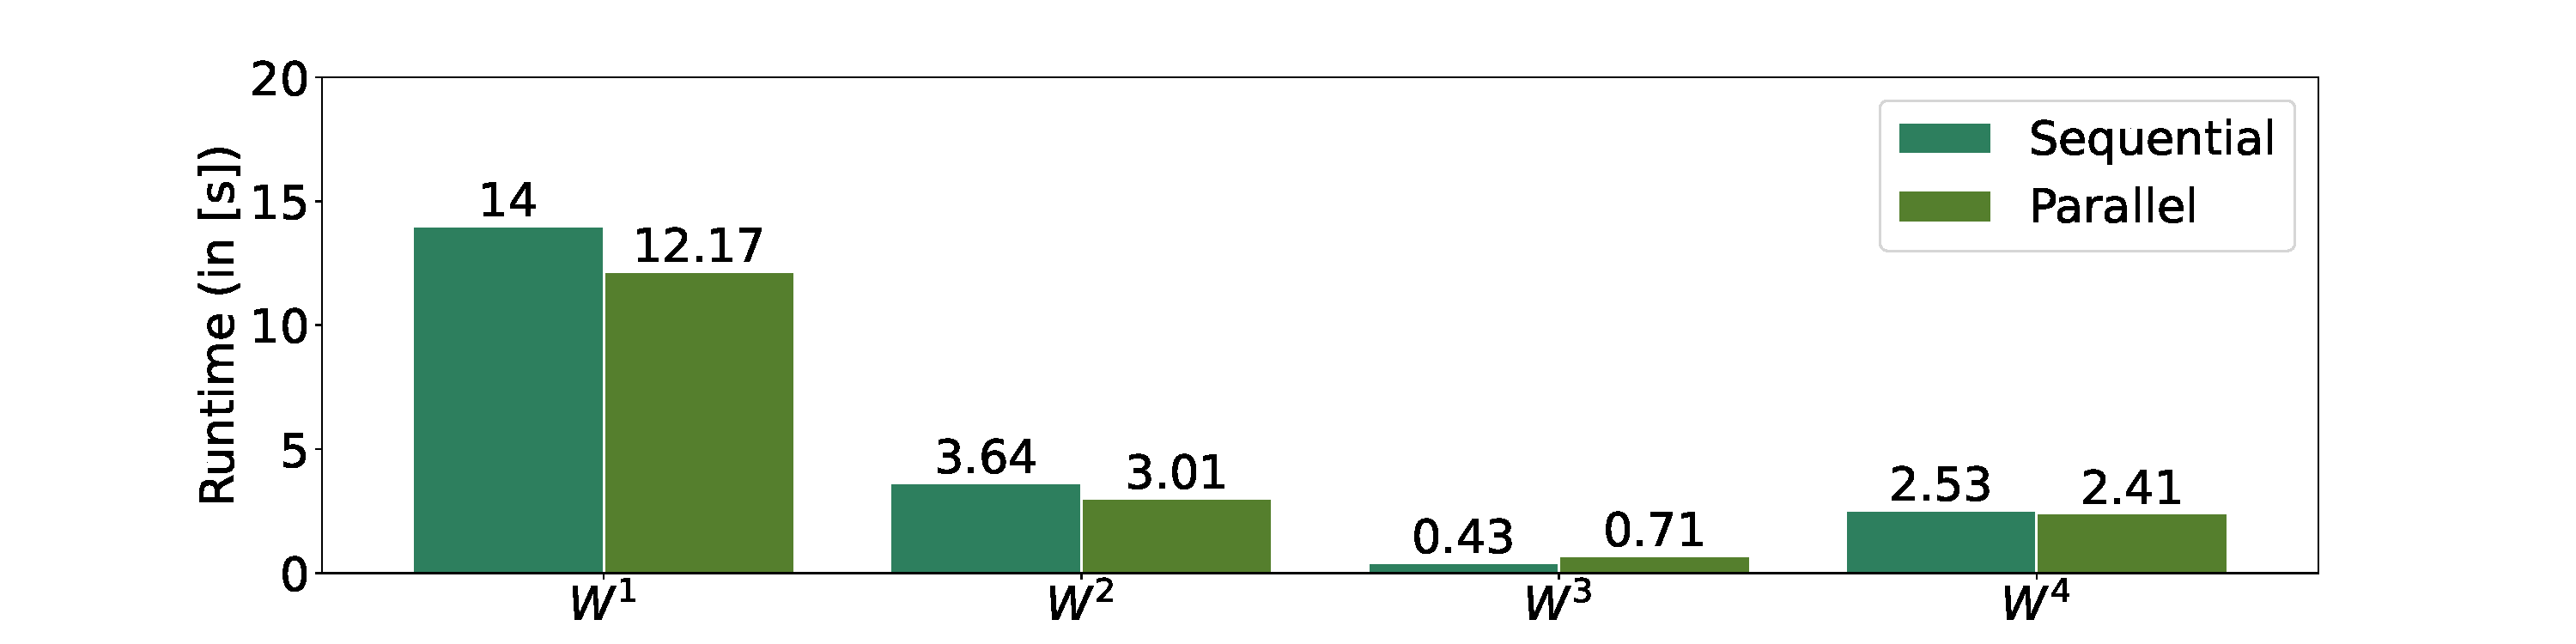
\includegraphics[width=\textwidth, trim = 0cm 1.5cm 0cm 1cm]{./plots/CGS_Performance.pdf}
\end{figure}

\subsection{Numerical Stability of CGS} \label{section:cgsStability}

CGS is in general said to be numerical unstable. The orthogonal projections of
the columns of $W$ are affected by rounding errors which accumulate for an
increasing column number $n$. In contrast to the Modified Gram-Schmidt algorithm
which will be discussed in the next section, CGS does not correct errors from
previous steps.

\citeauthor{Grigori:2023} \cite{Grigori:2023} gives the following theoretical
bound on the loss of orthogonality: Assuming \linebreak $c_1(m,n) \kappa^2(W) u
< 1$, it holds $||I - Q^T Q||_2 = c_2(m,n) \kappa^2(W) u$ with $c_1(m,n),
c_2(m,n) = O(mn^2)$. In particular, the loss of orthogonality scales quadratic
with the condition $\kappa(W)$. In Table \ref{tab:errorOrthoCGS} we present the
orthogonality loss as well as $\kappa(Q)$ of sequential and parallel CGS
(Algorithms \ref{cgs:sequential} and \ref{cgs:parallel}) for our four test
matrices.
\begin{table}[t]
    \centering
    \caption{Orthogonality loss $||I - Q^T Q||_2$ of CGS} \label{tab:errorOrthoCGS}
    \renewcommand{\arraystretch}{1.2}
    \begin{tabular}{|p{1.5cm}|c|c|c|c|c|c|c|c|}
      \hline
      \multirow{2}{1cm}{\textbf{Algorithm}} & \multicolumn{2}{c|}{$\textbf{W}^1$} &
      \multicolumn{2}{c|}{$\textbf{W}^2$} & \multicolumn{2}{c|}{$\textbf{W}^3$} &
      \multicolumn{2}{c|}{$\textbf{W}^4$}\\
      \cline{2-9}
      & loss & $\kappa(Q)$ & loss & $\kappa(Q)$
      & loss & $\kappa(Q)$ & loss & $\kappa(Q)$\\
      \hline
      Sequential    & $352.4$ & $6.5 \cdot 10^{16}$ & $2.9 \cdot 10^{-14}$ & 1
                        & $992.7$ & $2.2 \cdot 10^{22}$ & $3.4$ & $16 \cdot 10^4$ \\ \hline
      Parallel      & $408.5$ & $7.7 \cdot 10^{16}$ & $4.2 \cdot 10^{-14}$ & $1$
                        & $992.3$ & $3 \cdot 10^{20}$ & $3.5$ & $3.5 \cdot 10^4$ \\ \hline
    \end{tabular}
  \end{table}
Nevertheless, our test matrices are not well-suited to demonstrate that our
algorithms match $||I - Q^T Q||_2 = O(\kappa^2(W) u)$ because they vary in size
and condition at the same time. For this reason, we introduce a procedure
presented in \cite{Swirydowicz:2020} to generate matrices $W \in \mathbb{R}^{m
\times n}$ with condition number ranging from $1$ to $10^{15}$ and having the
same size: We set $W = U D V^T$ where $U \in \mathbb{R}^{m \times n}$ and $V \in
\mathbb{R}^{n \times n}$ are obtained by computing the $QR$ factorization of
normally distributed random matrices. The diagonal matrix $D \in \mathbb{R}^{n
\times n}$ has the following elements
\begin{equation*}
    D = \text{diag} (d_1, \ldots, d_n), \quad d_i = 10^{\alpha (i-1)}, \quad
    \alpha = \frac{\log_{10}\kappa(W)}{m - 1}.
\end{equation*}
As matrix dimensions, we chose $m = 2000$ and $n = 200$. By varying the value of
$\kappa(W)$ we obtain a sequence of matrices with the desired conditions in
$[1,10^{15}]$.

Figure \ref{fig:orthoErrorCGS} shows the orthogonality loss as well as the
condition of the orthonormal basis $Q$ of sequential and parallel CGS
(Algorithms \ref{cgs:sequential} and \ref{cgs:parallel}) for these test
matrices. The green line in the plot on the left illustrates $\kappa^2(W) u$ as
a reference. For $\kappa(W) \leq 10^9$ both algorithms perfectly match the
theoretical prediction and for $\kappa(W) > 10^9$ they perform even better. One
reason for the mismatch might be that the bound given by \cite{Grigori:2023}
holds only for $c_1(m,n) \kappa^2(W) u < 1$. Moreover, the same phenomenon could
be observed in \cite{Swirydowicz:2020}. In the plot on the right, we can see
that $\kappa(Q)$ is strongly dependent on $\kappa(W)$. Finally, note that as
expected sequential and parallel CGS produce almost the same results.
\begin{figure}[t]
    \centering
    \caption{CGS - Orthogonality loss and $\kappa(Q)$ as function of $\kappa(W)$} \label{fig:orthoErrorCGS}
    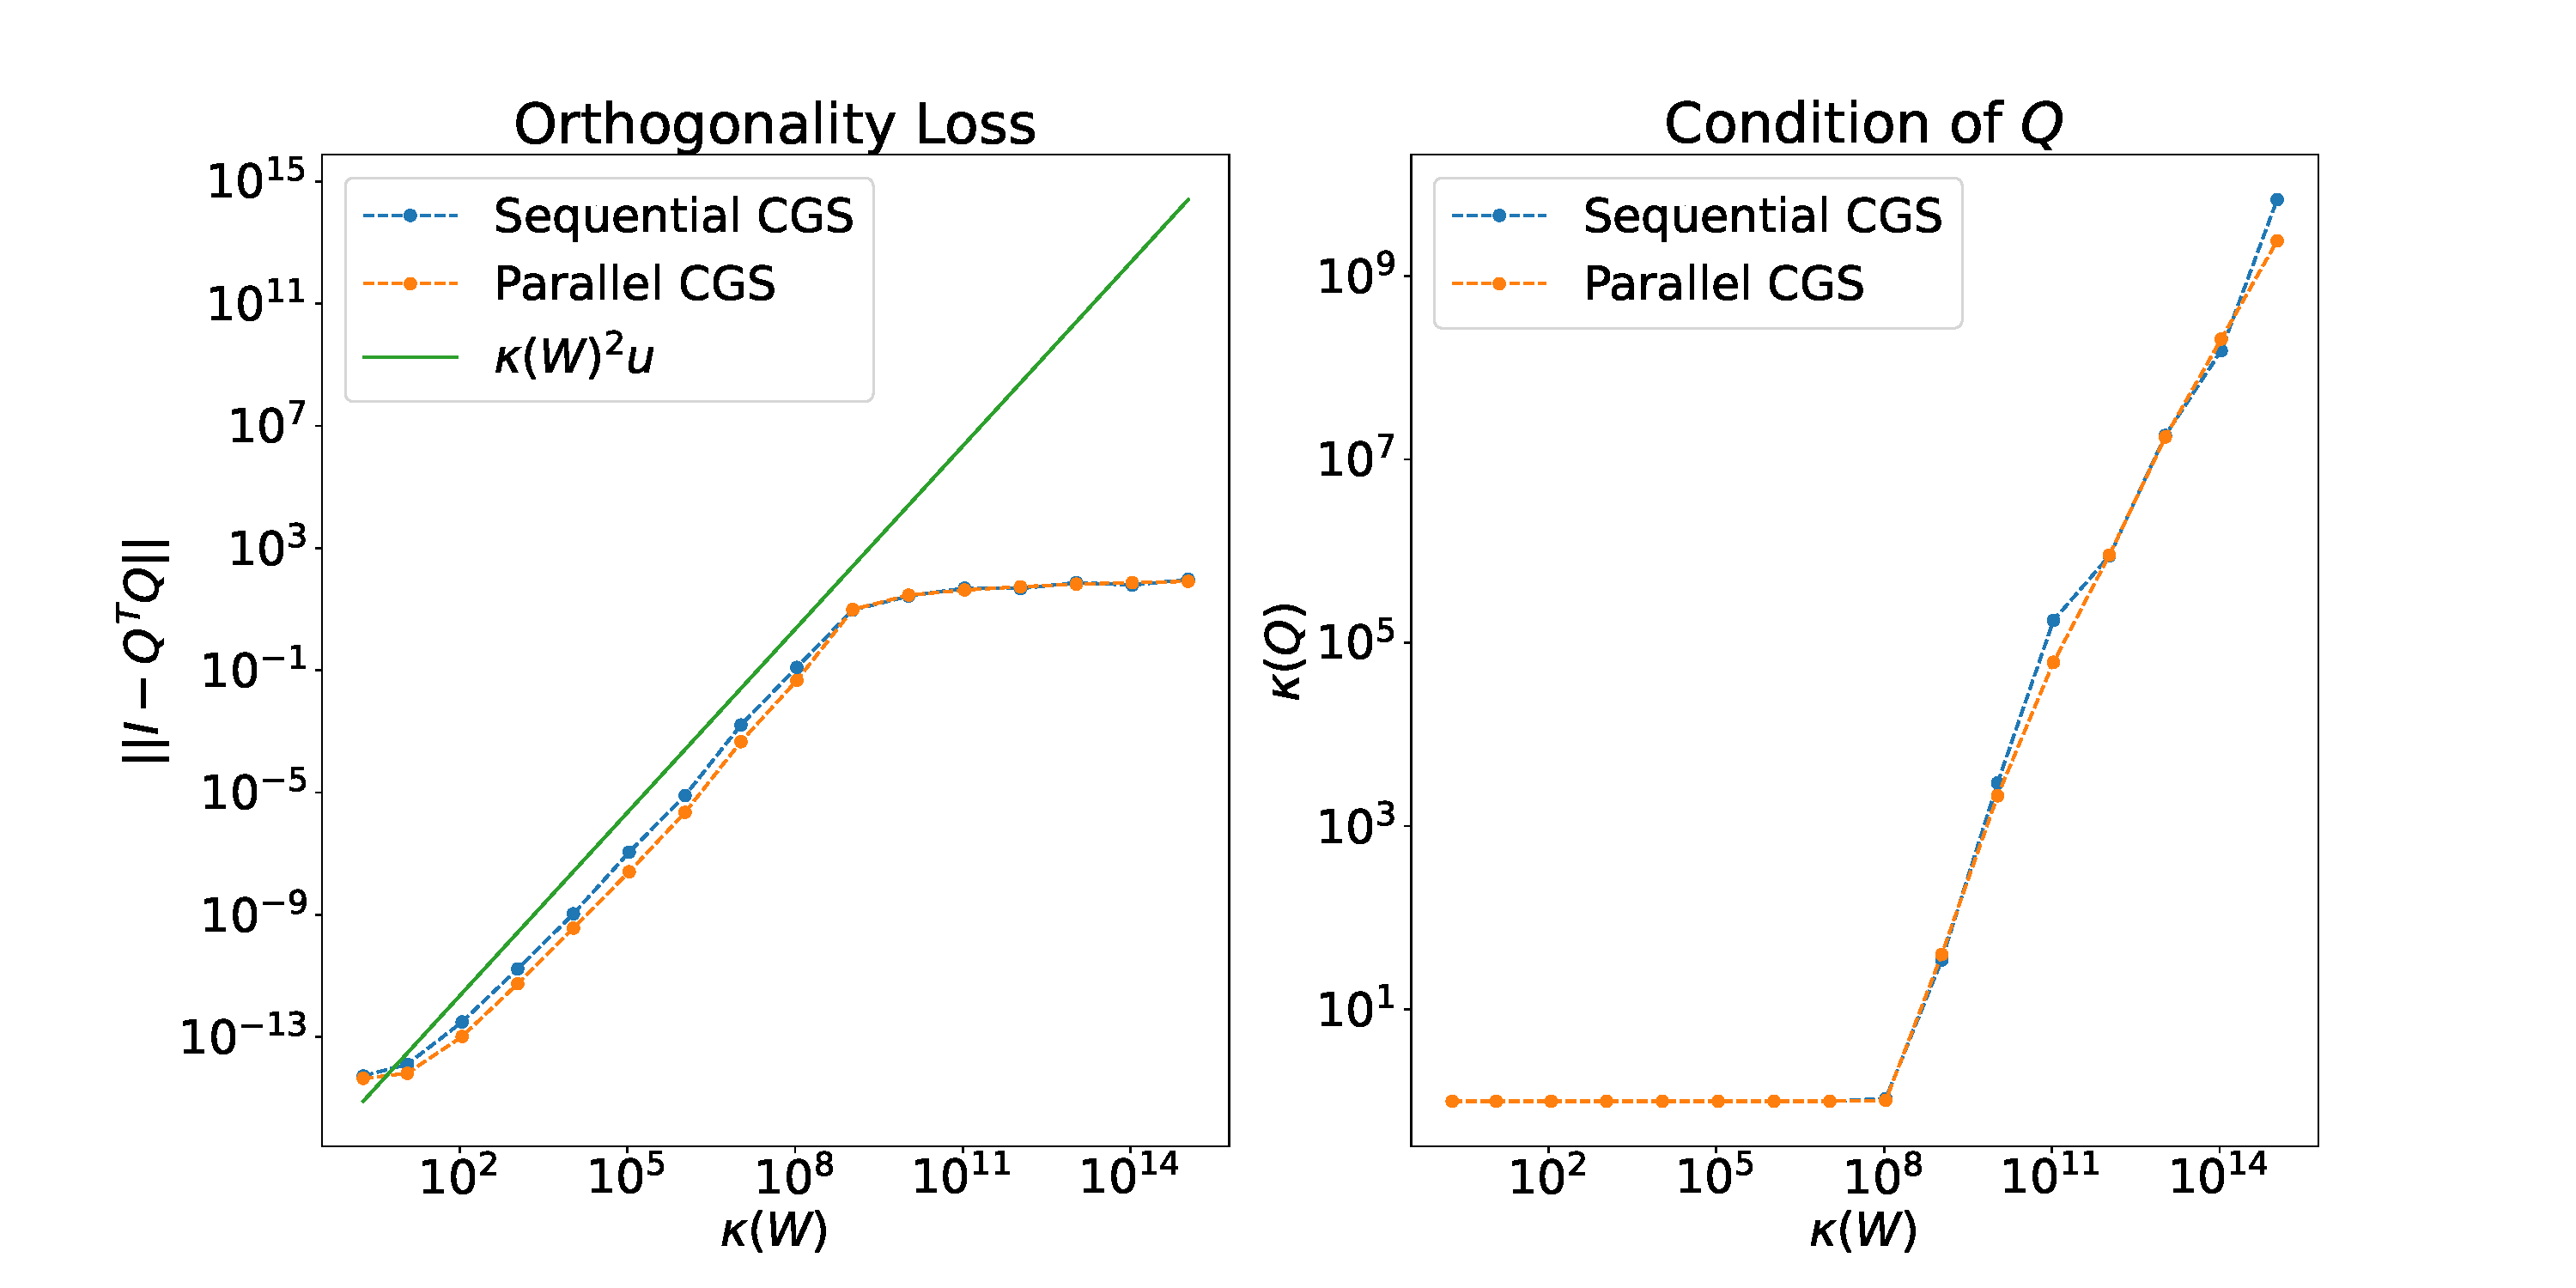
\includegraphics[width=\textwidth, trim = 0cm 1cm 0cm 1cm]
        {./plots/CGS_Orthogonality_Error_complete.pdf}
\end{figure}

In order to investigate the evolution of the orthogonality error $||I - Q^T
Q||_2$ and the condition of the orthonormal basis $Q$, we measured both in each
iteration of the CGS algorithms. Figure \ref{fig:numAnaCGS} illustrates our
results for $W^1,W^2,W^3,W^4$. The lines corresponding to each matrix stop at
different iterations because they differ in the number of columns. Once again,
both algorithms behave quite similarly. While the orthogonality errors of $W^1,
W^2$ are at a very high level from the first iterations onwards, the error of
$W^4$ jumps only in the last iterations. As expected, for the well-conditioned
matrix $W^2$ the orthogonality error and condition of $Q$ stay very small.
Finally, note that for all matrices $\kappa(Q)$ is at a similar level as
$\kappa(W)$ throughout the iterations.

\begin{figure}[t]
    \centering
    \caption{Numerical Analysis of CGS} \label{fig:numAnaCGS}
    \vspace*{-3mm}
    \begin{subfigure}{15cm}
        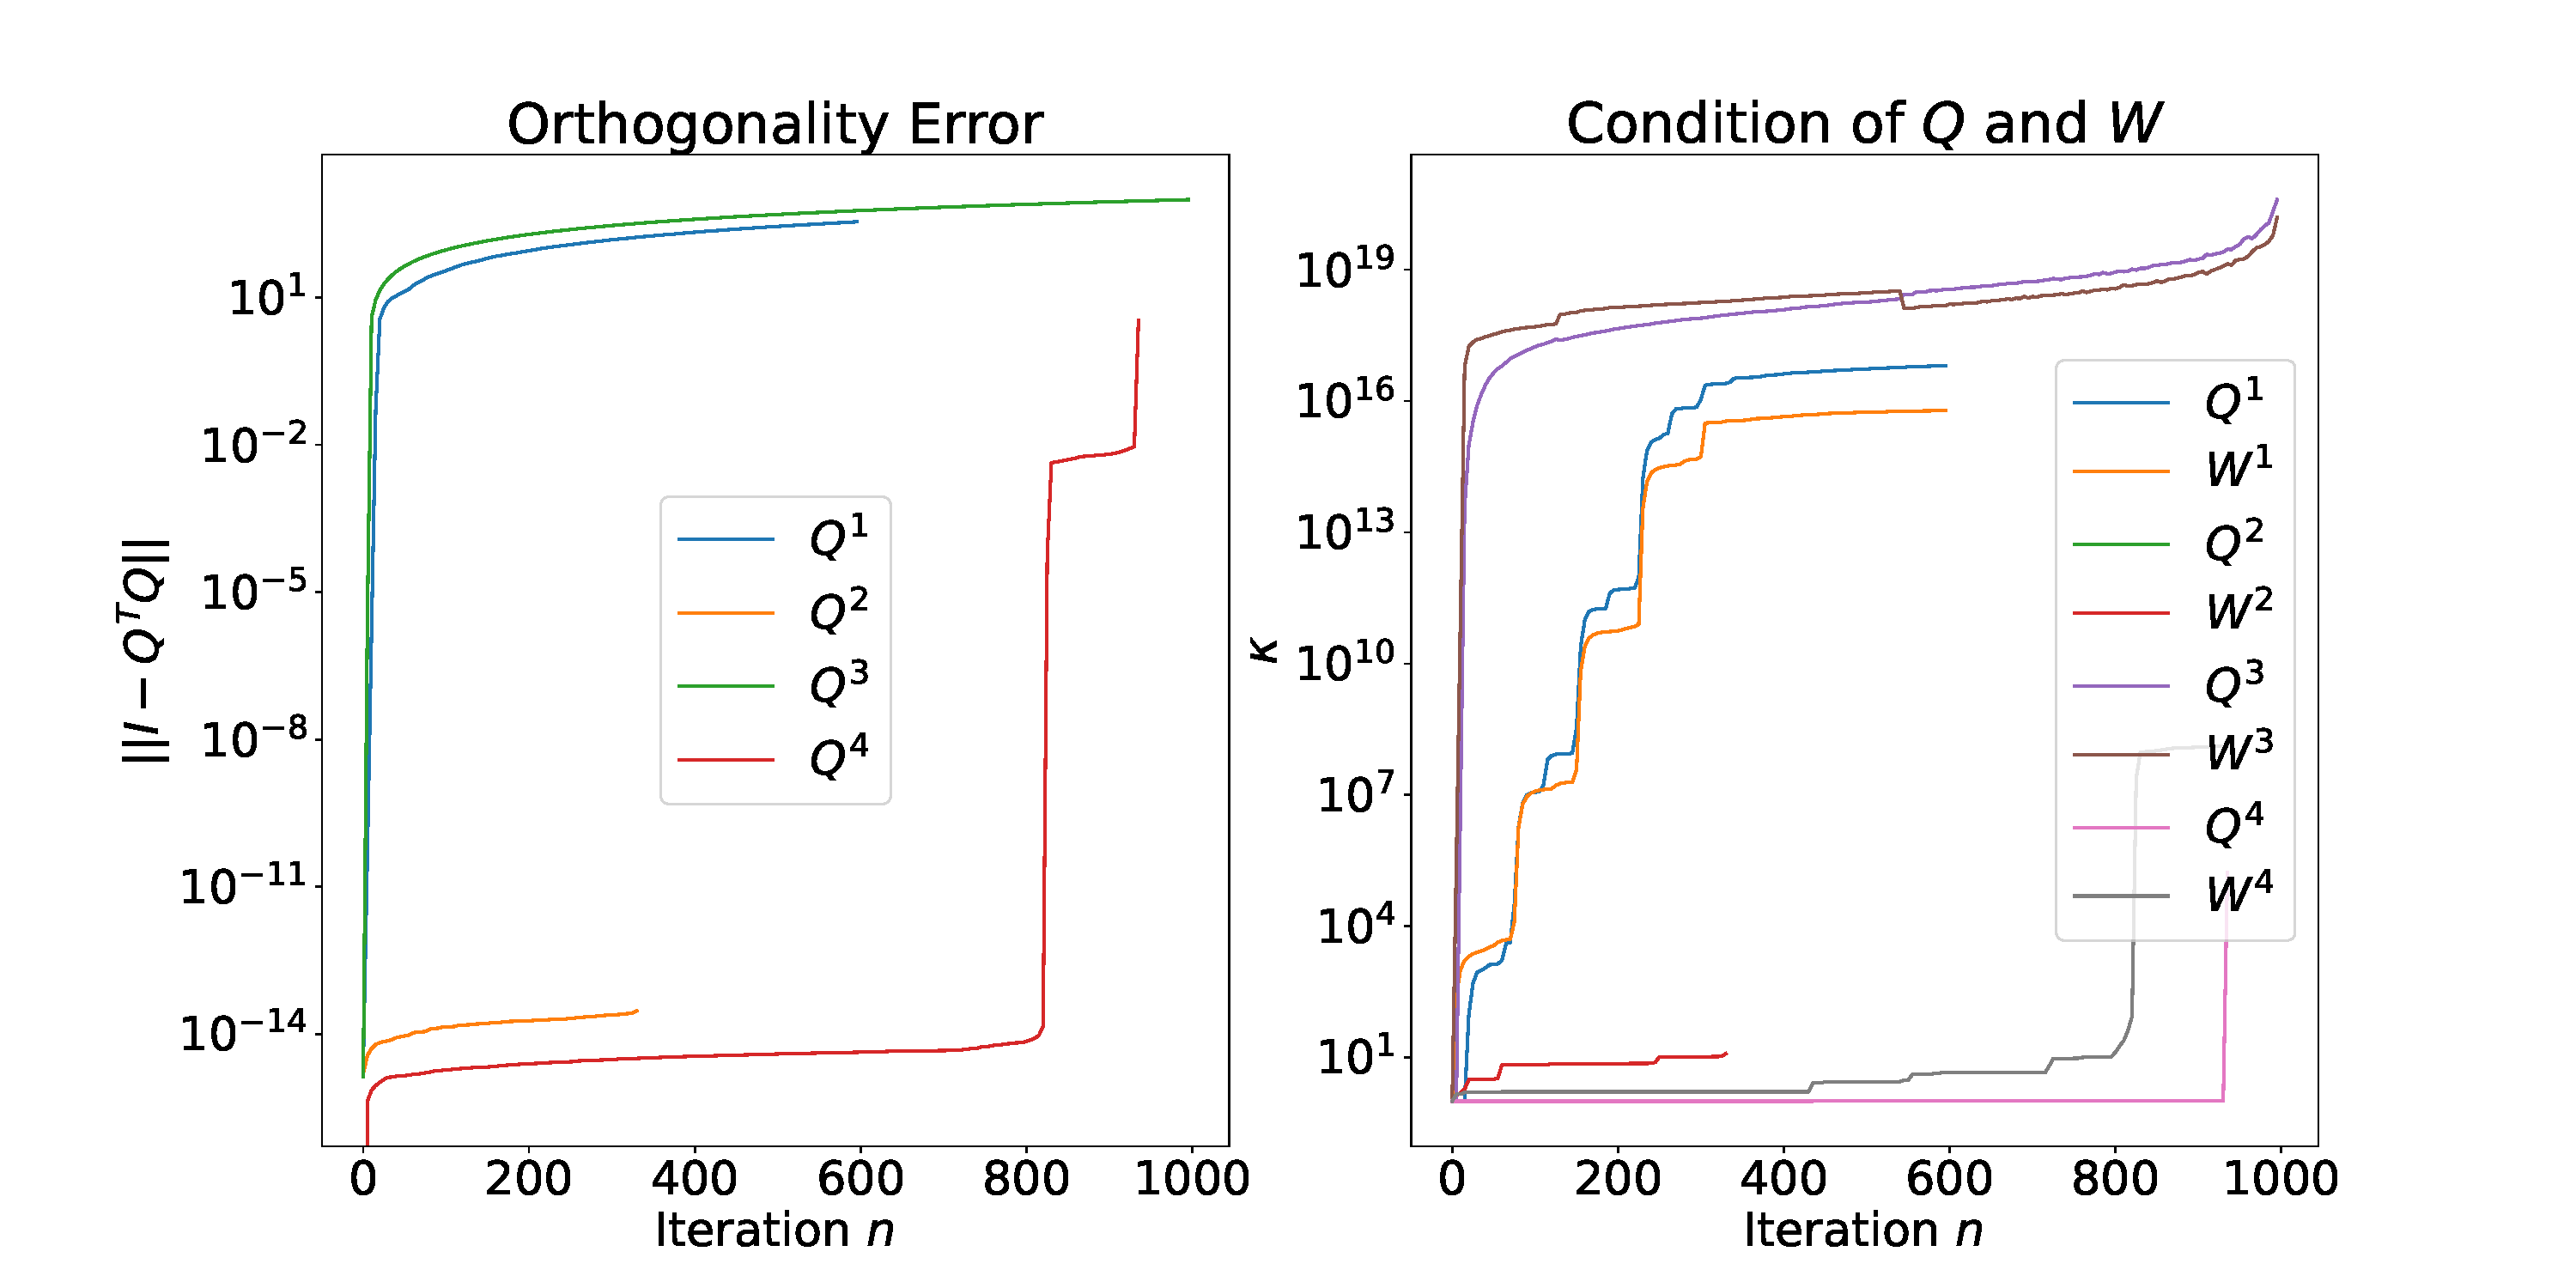
\includegraphics[width=\textwidth]{./plots/CGS_Numerical_Stability_Sequential_complete.pdf}
        \caption{Sequential CGS}
    \end{subfigure}\\
    \vspace*{-3mm}
    \begin{subfigure}{15cm}
        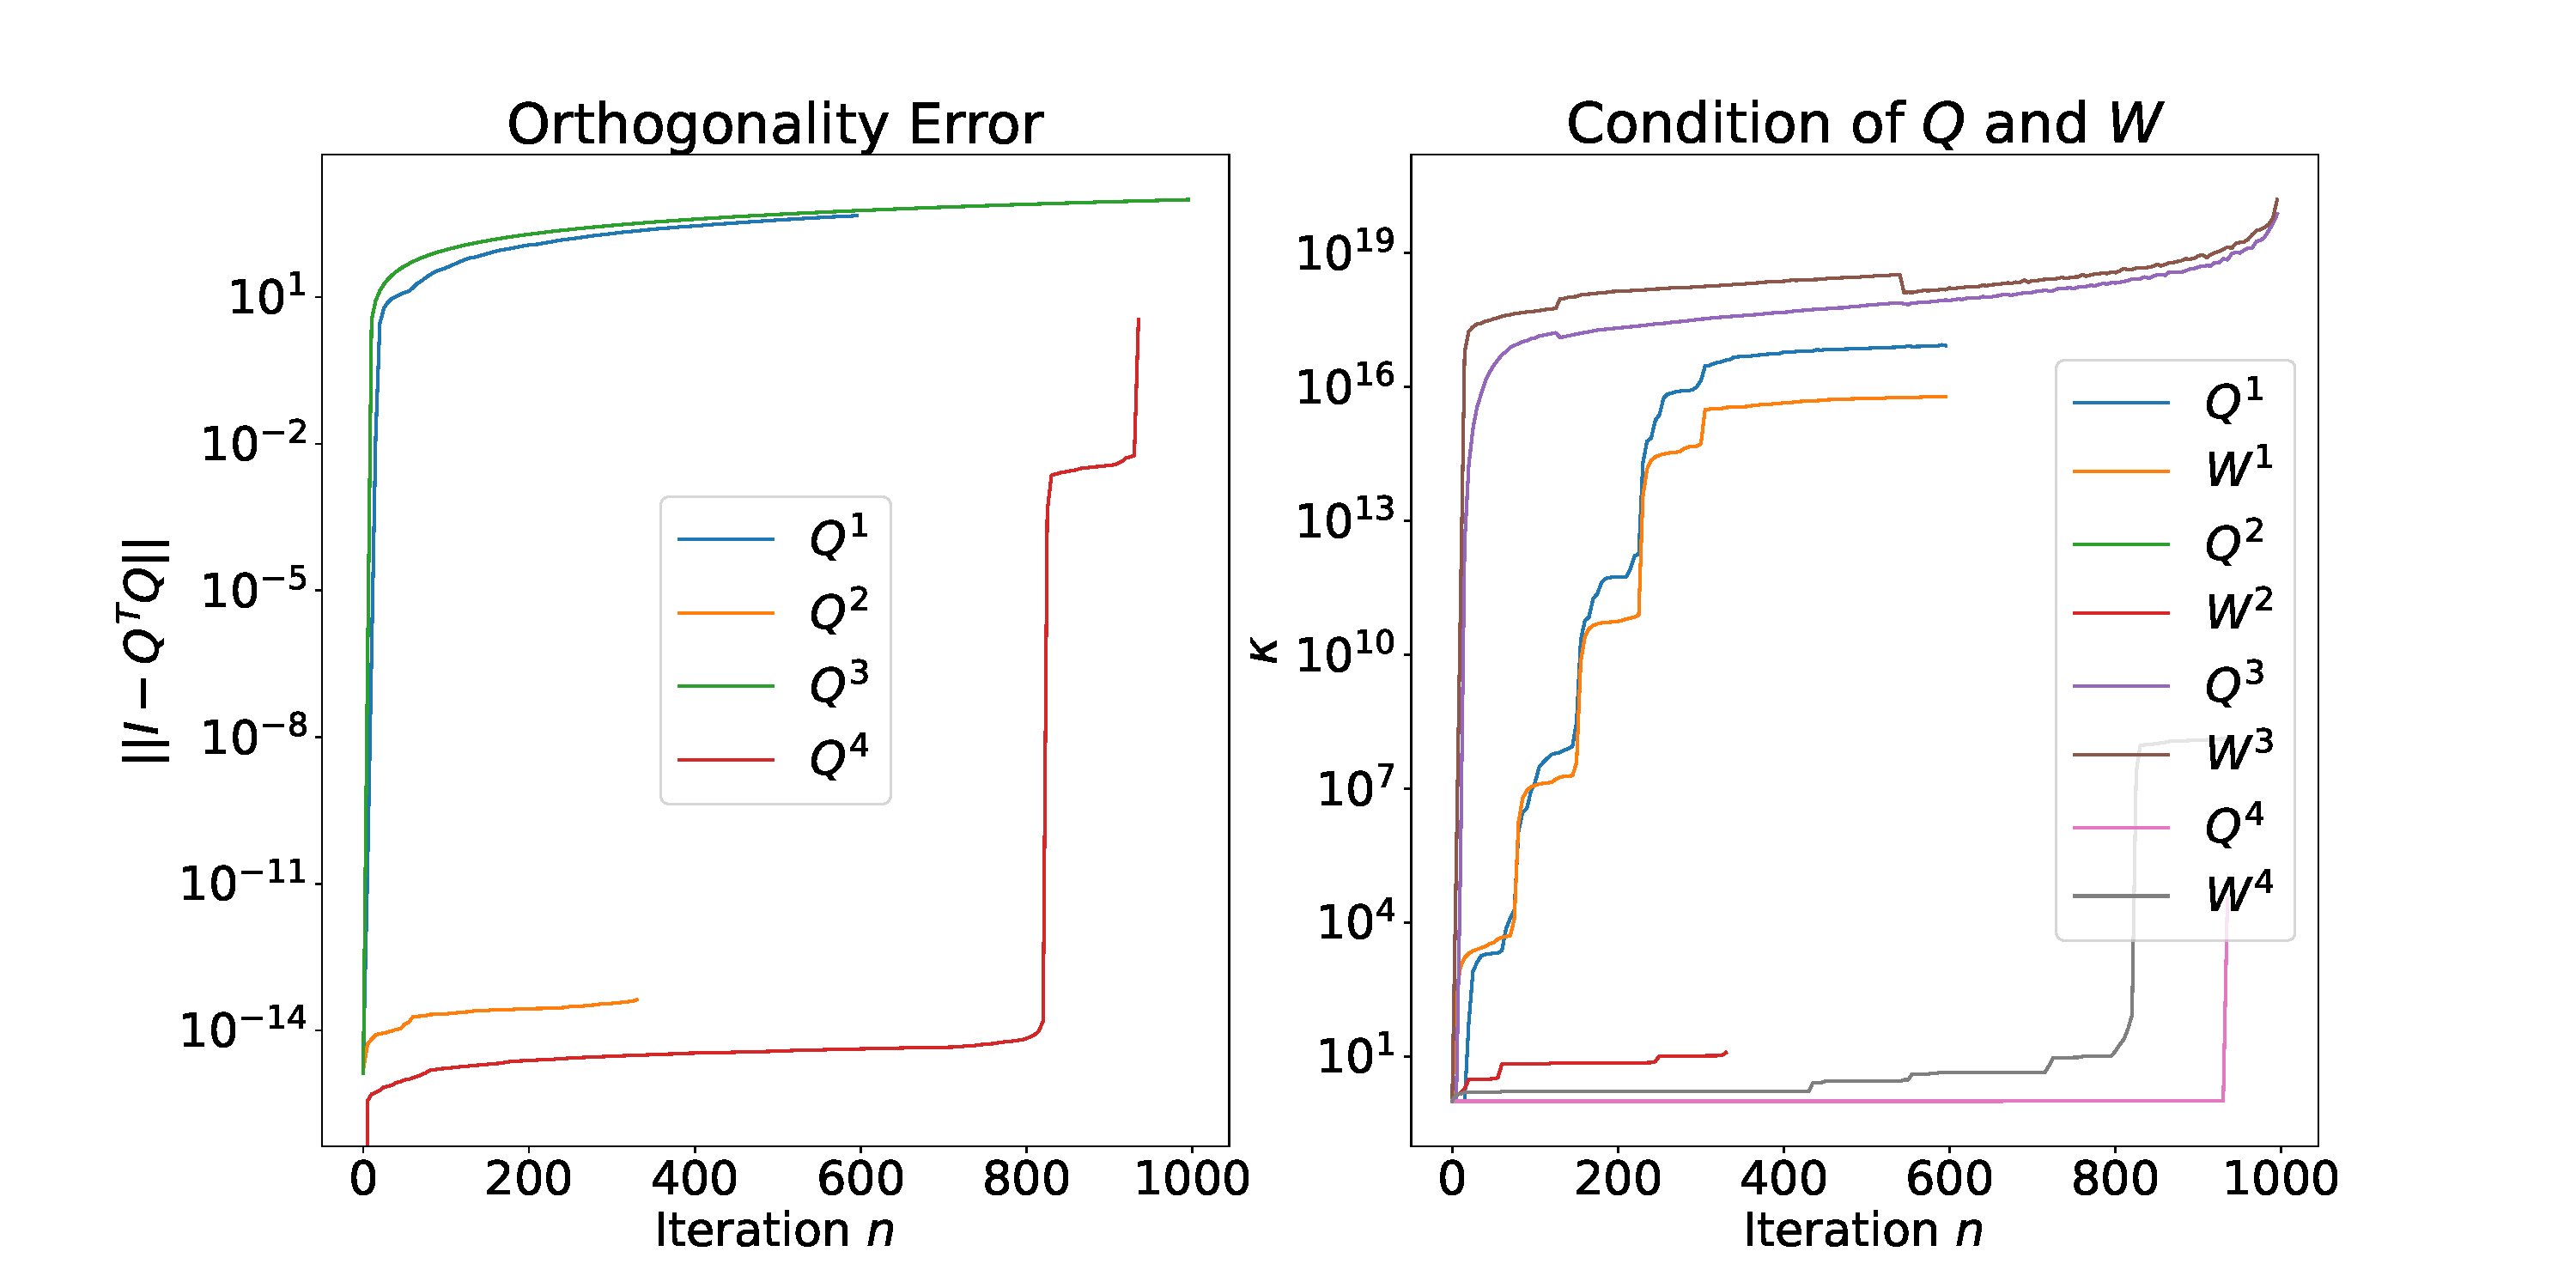
\includegraphics[width=\textwidth]{./plots/CGS_Numerical_Stability_Parallel_complete.pdf}
        \caption{Parallel CGS}
    \end{subfigure}
\end{figure}

\section{Modified Gram-Schmidt (MGS)}

The Modified Gram-Schmidt algorithm is mathematically equivalent to the
previously presented Classical Gram-Schmidt method. However, the involved
matrix-vector operations are rearranged in order to improve numerical stability
and avoid round-off errors. The MGS constructs an orthogonal set of vectors from
the columns of the given matrix $W$ through an iterative process of modifying
all forthcoming vectors to be orthogonal to the already computed ones. In
particular, in each step vectors are orthogonalized based on the previous
orthogonalization. This is the major difference compared to CGS and allows
correcting for rounding errors. The $i$-th iteration of the MGS is:
\begin{align}
    \begin{split}
        r_{ij} &:= \frac{w_i^T w_j}{|| w_i ||_2}
        \quad \quad \ \ \quad \forall j \in \{i, \ldots, n\} \\
        q_j &:= w_j - r_{ij} w_i \quad \quad \forall j \in \{i+1, \ldots, n\} \\
        q_i &:= \frac{w_i}{r_{ii}}
    \end{split}
\end{align}
where $w_i$ is the $i$-th column of $W$. The matrix $R \in \mathbb{R}^{n \times
n}$ of the $QR$ decomposition can be retrieved by the corresponding multipliers
$r_{ij}$. The pseudo-code for the sequential MGS can be found in Algorithm
\ref{mgs:sequential}. Similar to the implementation of CGS, the algorithm works
in-place and therefore the matrix $Q$ is stored within $W$. Again, we work only
with vectors and matrices instead of scalars to exploit the BLAS-routines. Note,
Algorithm \ref{mgs:sequential} is the \textit{right-looking} variant of MGS and
exclusively matrix-vector operations are used. Therefore only Level-2 BLAS
routines can be leveraged. However, there are indeed more complex reformulations
of MGS that use CGS as a subroutine to access Level-3 BLAS routines
\cite{GudulaSchwind:2005}. As the algorithm for CGS, Algorithm
\ref{mgs:sequential} requires $2mn^2$ floating-point operations. Nevertheless,
the concept of modifying all forthcoming vectors in each iteration causes
additional overhead and therefore MGS is not as efficient as CGS.
\begin{algorithm}[t]
    \caption{Sequential MGS} \label{mgs:sequential}
    \begin{algorithmic}[1]
        \For{{$i = 1$ to $n$}}
            \State $R[i,i] = || \ W[:,i] \ ||_2$
            \State $W[:,i] = W[:,i] / R[i,i] $
            \If{$i < n$}
                \State $R[i,i+1:n] = W[:,i]^T W[:,i+1:n]$
                \State $W[:,i+1:n] = W[:,i+1:n] - W[:,i] R[i,i+1:n]^T$
            \EndIf
        \EndFor
        \State \Return $W, R$
    \end{algorithmic}
\end{algorithm}

\subsection{Parallelization of MGS}
As for the CGS, the main problem when parallelizing MGS is the computation of
the norm of each vector and its inner product with subsequent vectors. Since we
use a row distribution for parallelization, a process of accumulating the inner
products across processors and making these known globally is necessary.

In Algorithm \ref{mgs:parallelized} we managed to reduce the communication
across processors to a \textit{reduce} and a \textit{broadcast} operation per
iteration. Therefore, we have $\# \ \text{messages} \ \dot{=} \ 2n \log(P)$ and
this is indeed the lower bound for the number of messages for (right-looking)
MGS \cite{Grigori:2008}. Recall that this is only half of the number of messages
we needed for the parallelized CGS. To achieve this, Algorithm
\ref{mgs:parallelized} reorders the operations of Algorithm
\ref{mgs:sequential}. First of all, row-blocks $B \in \mathbb{R}^{\frac{m}{P}
\times n}$ of the matrix $W \in \mathbb{R}^{m \times n}$ are scattered across
the available processors $P$. After that, each processor iterates over the
columns of its local block $B$. The algorithm computes $R[i,i:n] = (W[:,i]^T
W[:,i+1:n]) / ||W[:,i]||_2$ by calculating $B[:,i]^T B[:,i:n]$ locally, then
summing those vectors across processors via a reduce and finally broadcasting
the normed vector back. The rest of the computation can be done locally. The
final matrix $Q$ stored in $W$ must be retrieved by gathering all local blocks
back together. Note that the matrix $R$ is computed and stored by each processor
redundantly.

\begin{algorithm}[t]
    \caption{Parallelized MGS} \label{mgs:parallelized}
    \begin{algorithmic}[1]
        \State \Call{MPI.Scatterv}{$W$, $B$, root $= 0$}
        \For{{$i = 1$ to $n$}}
            \State $v = B[:,i]^T B[:,i:n]$
            \State $v =$ \Call{MPI.reduce}{$v$, MPI.SUM, root $= 0$}
            \If{rank $== 0$}
                \State $v = v / \sqrt{v[1]}$
            \EndIf
            \State $v =$ \Call{MPI.bcast}{$v$, root $= 0$}
            \State $B[:,i] = B[:,i] \ / \ v[1]$
            \State $R[i,i:n] = v$
            \State $B[:,i+1:n] = B[:,i+1:n] - B[:,i] \ R[i,i+1:n]$
        \EndFor
        \State \Call{MPI.Gatherv}{$B$, $W$, root $= 0$}
        \State \Return $W, R$
    \end{algorithmic}
\end{algorithm}

\subsection{Performance Evaluation of MGS}

Now, let us compare the performance of the parallelized and the sequential MGS.
Figure \ref{fig:performanceMGS} shows the runtime of Algorithms
\ref{mgs:sequential} and \ref{mgs:parallelized} computing the $QR$ decomposition
of our four test matrices. Again, we computed both matrices $Q$ and $R$
explicitly, the illustrated runtimes are averages of $10$ code executions and we
executed the parallel MGS on all 4 available processors. The parallel algorithm
has significantly lower runtimes. In particular, we can see that Algorithm
\ref{mgs:parallelized} performs very well on the two tall and skinny matrices
$W^1$ and $W^2$. However, when it comes to small square matrices like $W^3$
(Hilbert matrix) the sequential algorithm matches almost the performance of the
parallelized version. Note that both algorithms are considerably slower than our
CGS algorithms.
\begin{figure}[t]
    \centering
    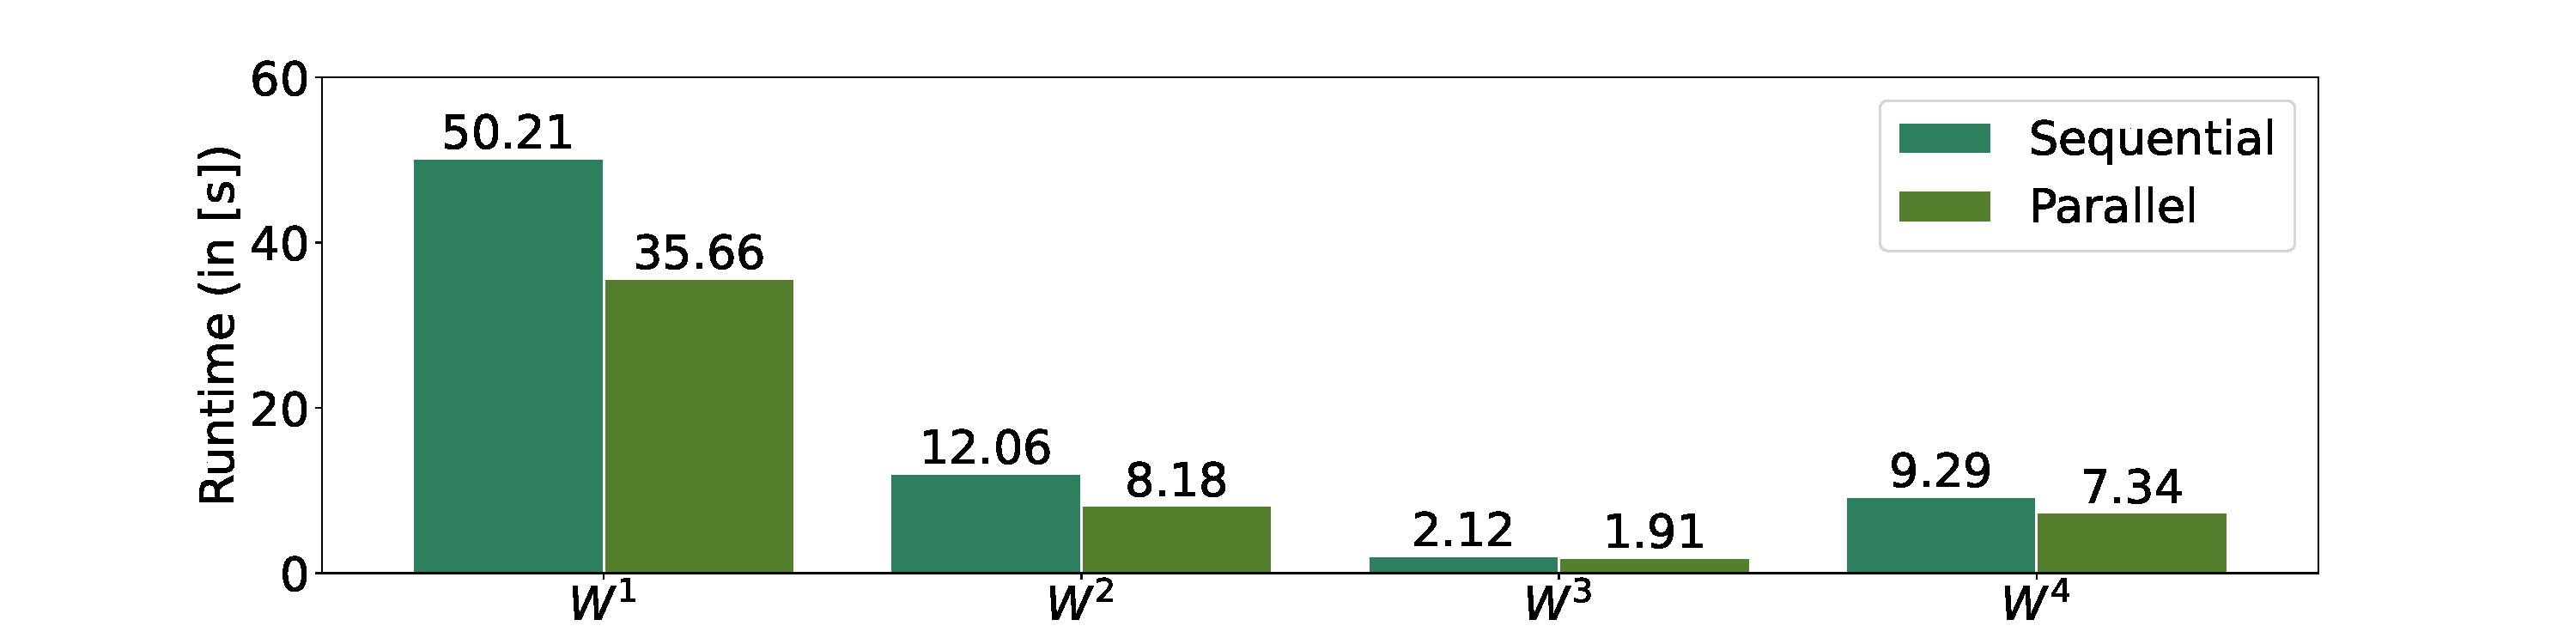
\includegraphics[width=\textwidth, trim = 0cm 1.5cm 0cm 1.25cm]{./plots/MGS_Performance.pdf}
    \caption{Runtime of sequential and parallel MGS} \label{fig:performanceMGS}
\end{figure}

\subsection{Numerical Stability of MGS}

In general, MGS provides backward stable solutions \cite{Bornemann:2018}.
Regarding the loss of orthogonality, \citeauthor{Grigori:2023}
\cite{Grigori:2023} gives the following bound: Assuming $c(m,b) \kappa(W) u <
1$, it holds $||I - Q^T Q||_2 = c(m,b) \kappa(W) u$ with $c(m,b) = O(mb)$.
Therefore, the orthogonality error of MGS scales only linearly w.r.t. the
condition $\kappa(W)$ and not quadratic as for CGS. Table
\ref{tab:errorOrthoMGS} shows the orthogonality loss as well as the condition
$\kappa(Q)$ for sequential and parallel MGS (Algorithms \ref{mgs:sequential} and
\ref{mgs:parallelized}).
\begin{table}[t]
    \centering
    \caption{Orthogonality loss $||I - Q^T Q||_2$ of MGS} \label{tab:errorOrthoMGS}
    \renewcommand{\arraystretch}{1.2}
    \begin{tabular}{|p{1.5cm}|c|c|c|c|c|c|c|c|}
      \hline
      \multirow{2}{1cm}{\textbf{Algorithm}} & \multicolumn{2}{c|}{$\textbf{W}^1$} &
      \multicolumn{2}{c|}{$\textbf{W}^2$} & \multicolumn{2}{c|}{$\textbf{W}^3$} &
      \multicolumn{2}{c|}{$\textbf{W}^4$}\\
      \cline{2-9}
      & loss & $\kappa(Q)$ & loss & $\kappa(Q)$
      & loss & $\kappa(Q)$ & loss & $\kappa(Q)$\\
      \hline
      Sequential    & $9.95$ & $9.54$ & $4.05 \cdot 10^{-14}$ & $1$
                        & $8.01$ & $21664.67$ & $2.82 \cdot 10^{-8}$ & $1$ \\ \hline
      Parallel      & $5.14$ & $3.49$ & $3.91 \cdot 10^{-14}$ & $1$
                        & $7.07$ & $12711.47$ & $2.34 \cdot 10^{-8}$ & $1$ \\ \hline
    \end{tabular}
  \end{table}

In Figure \ref{fig:orthoErrorMGS}, we plot the orthogonality loss of MGS for a
sequence of matrices generated by the procedure described in Section
\ref{section:cgsStability}. In the plot on the left, the green line shows
$\kappa(W) u$ as a reference. Both, sequential and parallel MGS (Algorithms
\ref{mgs:sequential} and \ref{mgs:parallelized}), match the predicted
orthogonality loss. It is noticeable that parallel MGS has a slightly smaller
orthogonality loss than the sequential one. In the plot on the right, we can see
that the condition of the input matrix $\kappa(W)$ has only a small impact on
$\kappa(Q)$.
\begin{figure}[t]
    \centering %
    \caption{MGS - Orthogonality loss and $\kappa(Q)$ as function of $\kappa(W)$} \label{fig:orthoErrorMGS}
    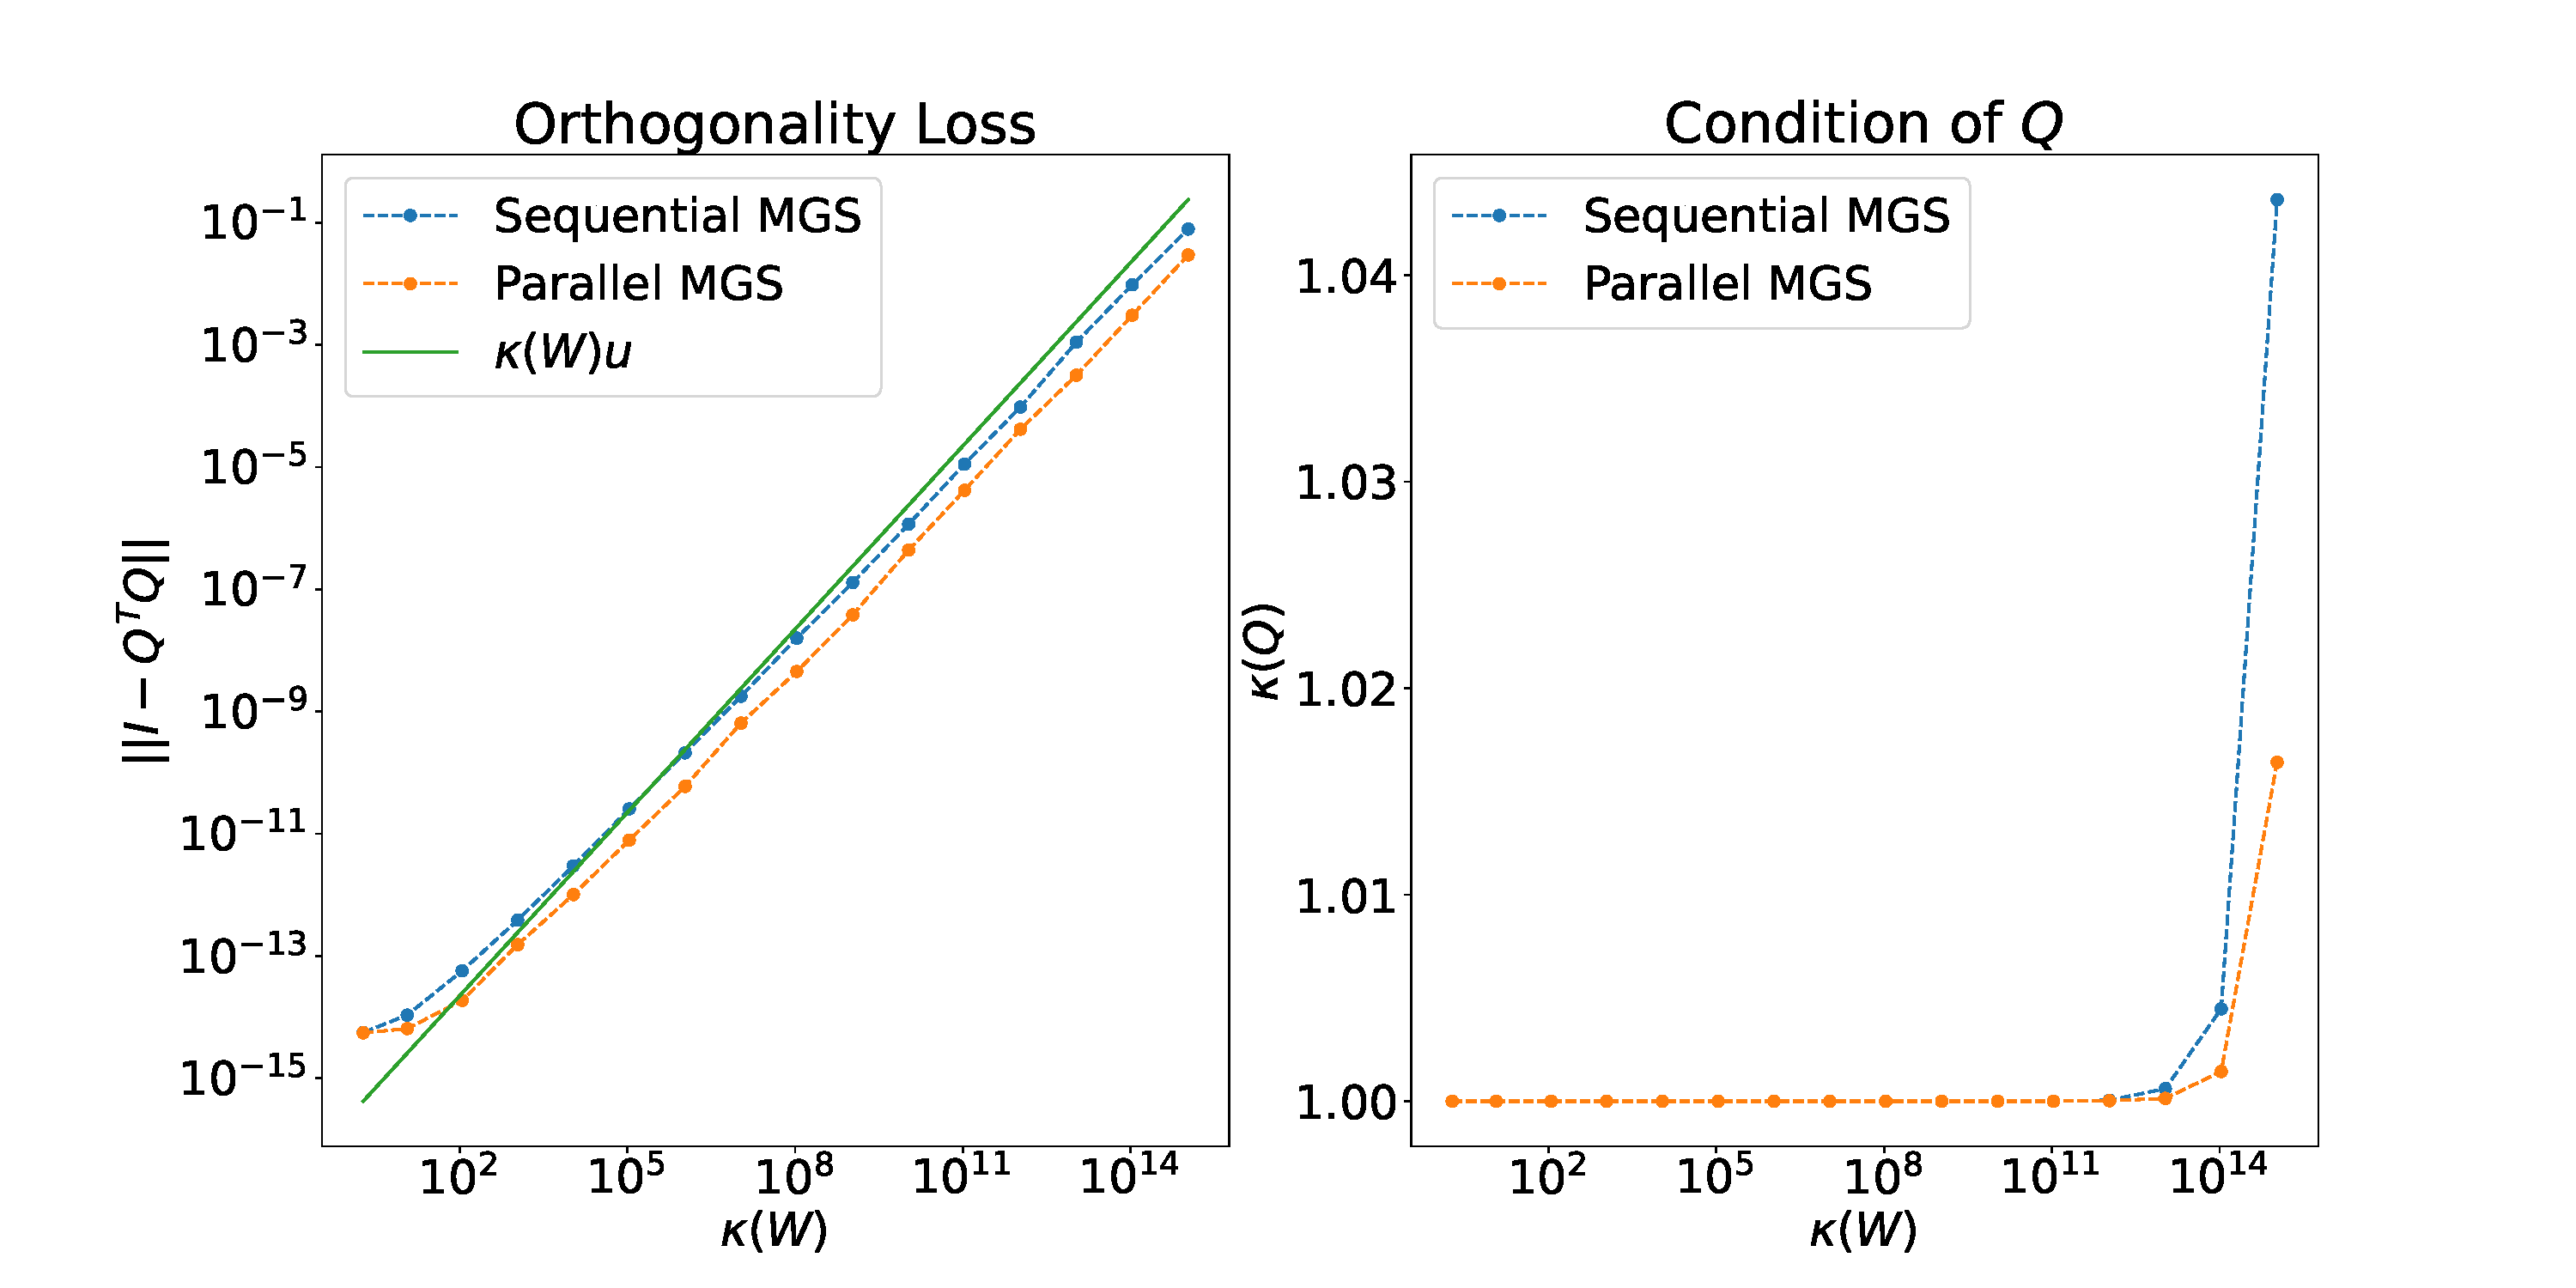
\includegraphics[width=\textwidth, trim = 0cm 1cm 0cm 1cm]{./plots/MGS_Orthogonality_Error_complete.pdf}
\end{figure}

Finally, Figure \ref{fig:numAnaMGS} shows the evolution of the orthogonality
loss $||I - Q^T Q||_2$ as well as the condition of the orthonormal basis $Q$ in
each iteration of Algorithms \ref{mgs:sequential} and \ref{mgs:parallelized} for
our four test matrices. Both algorithms behave similarly. The orthogonality loss
of $Q$ is slightly lower than in Figure \ref{fig:numAnaCGS} and the condition
$\kappa(Q)$ scales only slowly w.r.t. $\kappa(W)$. This is a massive improvement
compared to CGS and confirms the theory as well as our observations from Figure
\ref{fig:orthoErrorMGS}.
\begin{figure}[t]
    \centering
    \caption{Numerical Analysis of MGS} \label{fig:numAnaMGS}
    \vspace*{-3mm}
    \begin{subfigure}{15cm}
        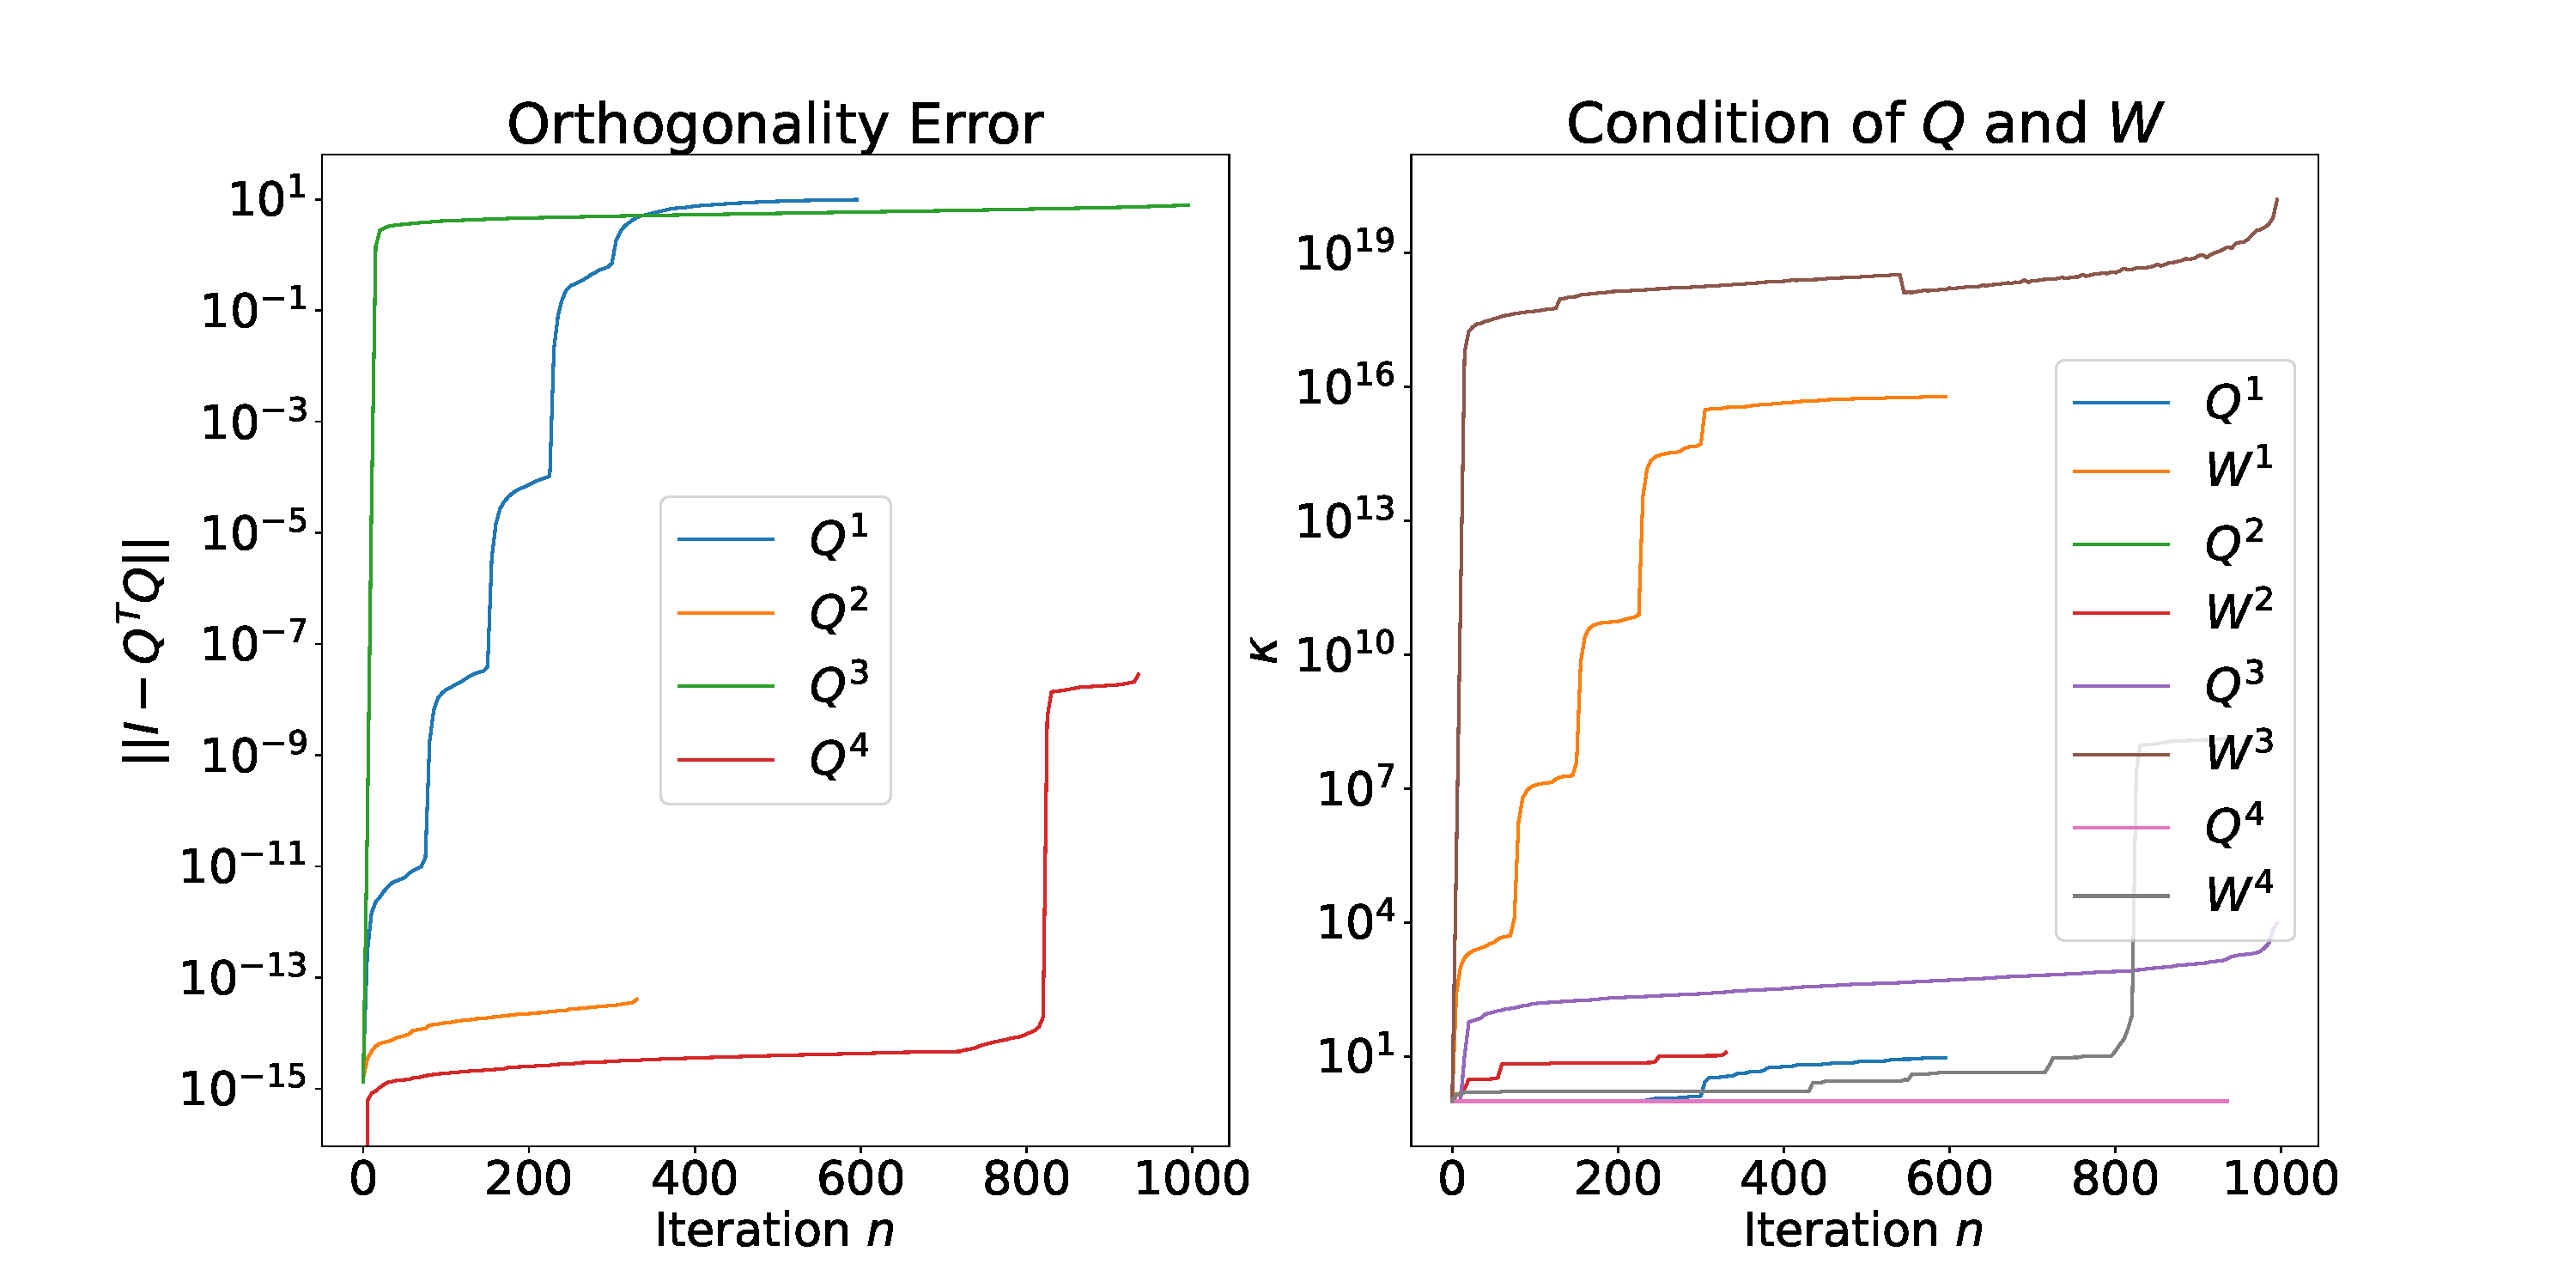
\includegraphics[width=\textwidth]{./plots/MGS_Numerical_Stability_Sequential_complete.pdf}
        \caption{Sequential MGS}
    \end{subfigure}\\
    \vspace*{-3mm}
    \begin{subfigure}{15cm}
        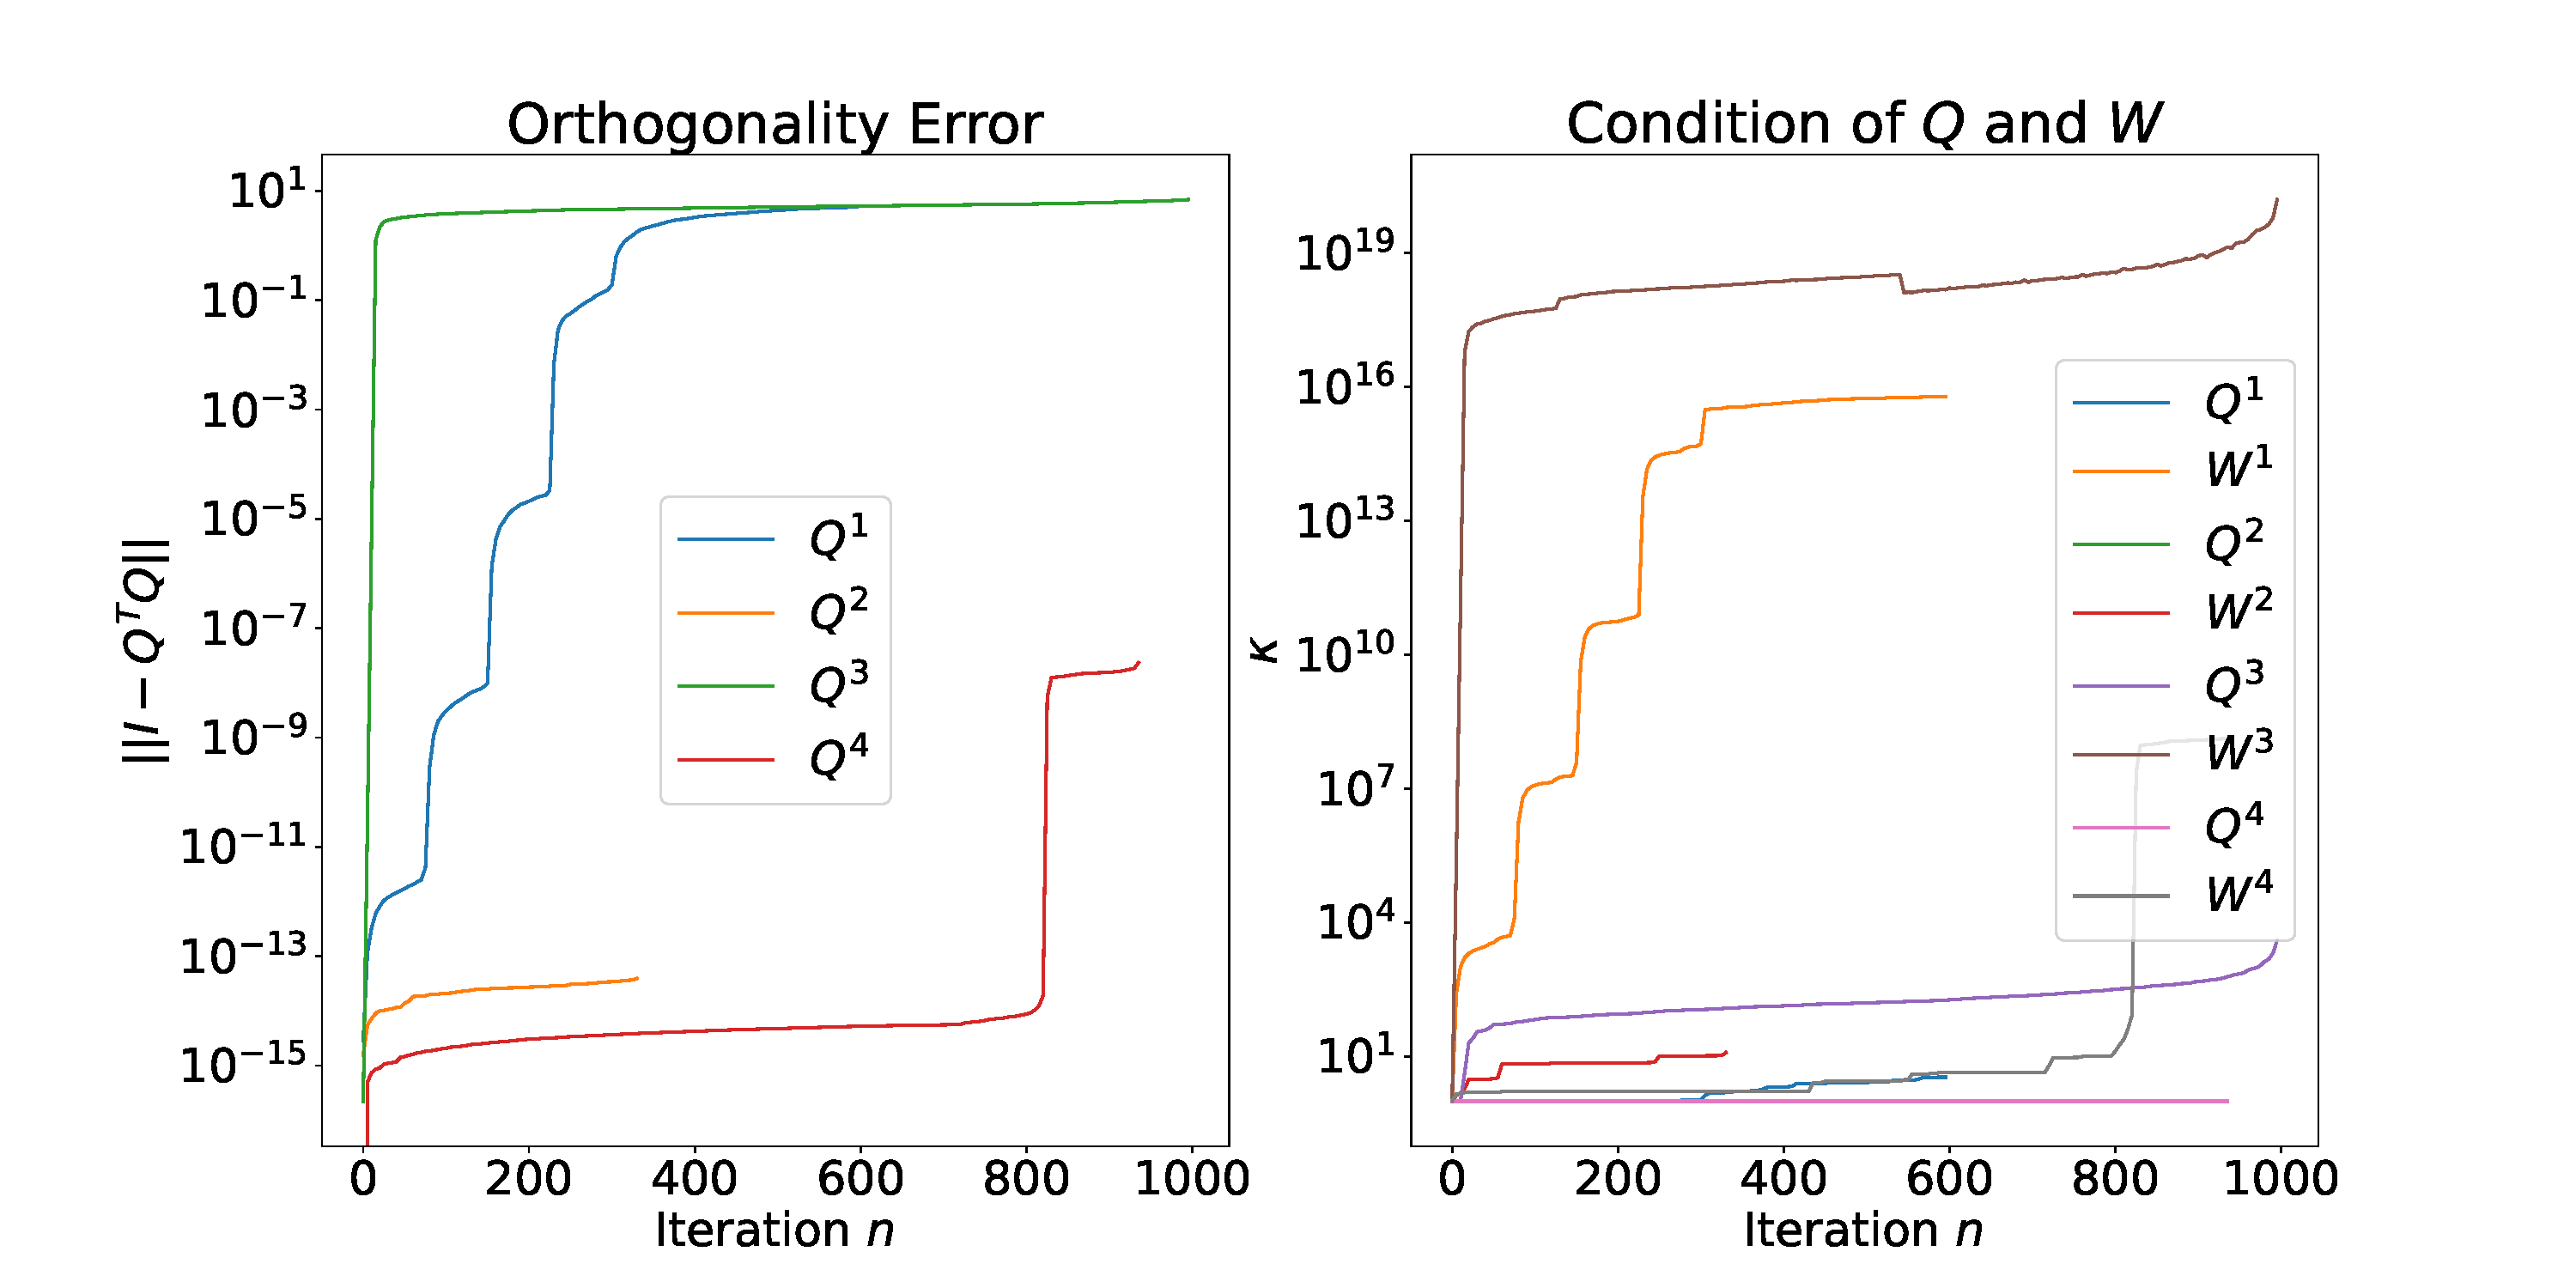
\includegraphics[width=\textwidth]{./plots/MGS_Numerical_Stability_Parallel_complete.pdf}
        \caption{Parallel MGS}
    \end{subfigure}
\end{figure}

\section{Tall Skinny QR (TSQR) Decomposition}

The tall skinny $QR$ (TSQR) decomposition of a matrix $W$ developed by
\citeauthor*{Grigori:2008} \cite{Grigori:2008} is a communication optimal $QR$
decomposition for matrices with many more rows than columns ($m \gg n$). The
basic idea is to use a reduction-like operation on a tree to compute the $QR$
factorization: First, the algorithm scatters $\frac{m}{P} \times n$ row-blocks
$B$ of the $m \times n$ matrix $W$ across $P$ processors. Second, the $QR$
decomposition is computed in each local block independently. Third, the
processors recombine the $R$ factors within each group of neighboring processors
and continue the process by communicating their $R$ factors to the next set of
neighbors. For an illustration, see \cite{Grigori:2008}. The major difference
between sequential and parallel TSQR is the underlying tree structure which is
used for the matrix factorization.

\subsection{Sequential TSQR}

Sequential TSQR uses a \textit{flat tree} or \textit{linear chain} for the
factorization process. As described above, we first divide the input matrix $W$
into row-blocks $B_i \in \mathbb{R}^{\frac{m}{P} \times n}$ with $i \in [P]$ and
compute the $QR$ decomposition of $B_1$. Then, we combine the factor $R_1$ with
$B_2$ by \textit{stacking} the two matrices on top of each other and compute the
$QR$ decomposition of $\left(\begin{smallmatrix} R_1 \\ B_2
\end{smallmatrix}\right)$. We continue this process until we run out of matrices
$B_i$. The $R$ factor of the final iteration is the $R$ factor of the $QR$
decomposition of $W$. The $Q$ factor can be retrieved by computing a specific
matrix product of the local $Q$ factors obtained in each iteration (for details
see \cite{Grigori:2008}). However, in practice, it is useful to store the local
$Q$ factors implicitly, analogous to using the Householder vectors computed by
Householder $QR$ as an implicit representation of the $Q$ factor. Algorithm
\ref{tsqr:sequential} illustrates the described procedure.

\begin{algorithm}[t]
    \caption{Sequential TSQR with implicitly stored $Q$} \label{tsqr:sequential}
    \begin{algorithmic}[1]
        \State $b = m / P$
        \State $B = W[1 : b, :]$
        \For{{$i = 1$ to $P$}}
            \If{$i > 1$}
                \State $B = \left(\begin{smallmatrix} R \\ W[(i-1) \cdot b : i \cdot b, :]
                \end{smallmatrix}\right)$
            \EndIf
            \State $Q_i, R =$ \Call{QR}{$B$}
        \EndFor
        \State \Return $R$
    \end{algorithmic}
\end{algorithm}

\subsection{Parallel TSQR}

Parallel TSQR fits into the same general framework as the sequential TSQR
decomposition. The difference is that we use a \textit{binary tree} instead of a
flat tree. In Algorithm \ref{tsqr:parallel}, we first divide the input matrix
$W$ into row-blocks $B_{p_i,0} \in \mathbb{R}^{\frac{m}{P} \times n}$ with $p_i
\in [P]$ and $0$ indicating the bottom tree level. Next, we compute the $QR$
decomposition of all local blocks $B_{p_i,0}$ in parallel and group the
resulting $R_{p_i,0}$ factors by stacking successive pairs
$\left(\begin{smallmatrix} R_{p_i,0} \\
R_{p_{i+1},0} \end{smallmatrix}\right)$. In the next iteration, we compute the
$QR$ decomposition of these pairs on $P / 2$ processors and recombine again. We
perform iterations until there is only one $R$ factor left. This is the root of
the binary tree and the $R$ factor of the $QR$ decomposition of $W$. The final
$Q$ can be computed explicitly based on the local $Q_{p_i,j}$ distributed across
the processors as shown in our Python implementation in Listing
\ref{python:parallelTSQR}. We simply traverse the binary tree backward,
splitting the matrix $Q_{p_i,j}$ into an upper and lower half $Q_{p_i,j} =
\left(\begin{smallmatrix} Q_{p_iu,j} \\ Q_{p_il,j} \end{smallmatrix}\right)$ at
each tree level $j$. The lower half $Q_{p_il,j}$ is sent to a neighboring
processor $p_k$ and the two matrix-matrix products $Q_{p_i,j-1} \cdot
Q_{p_iu,j}$, $Q_{p_k,j-1} \cdot Q_{p_il,j}$ are computed in parallel. At the
bottom tree level, the local $Q$ products are gathered together and the
resulting matrix is the $Q$ factor of the $QR$ decomposition of $W$. This
backward traversal is advantageous compared to computing $Q$ in the same
iterations as $R$ because of reduced matrix dimensions. $Q_{i,0}$ has dimensions
$\frac{m}{P} \times n$ and $Q_{i,j}$ for $j > 1$ has dimensions $2n \times n$.
If we started computing $Q$ at the tree leaves, we would have to compute the
matrix product of a $\frac{m}{P} \times n$ and a $n \times n$ matrix in each
iteration. In contrast, if we start computing $Q$ at the tree root, we only need
to calculate the matrix product two $n \times n$ matrices until the very last
iteration (in which we have to face a matrix product of a $\frac{m}{P} \times n$
and a $n \times n$ matrix).

In practice, however, it is preferable to store $Q$ implicitly. Note that a
binary tree and therefore our algorithm works only for the number of processes
$P$ being a power of $2$. Finally, it holds $\# \ \text{messages} \ \dot{=} \
\log(P)$ for parallel TSQR and the number of messages does in particular not
depend on the matrix size. Therefore, the algorithm scales very well for large
matrices.
\begin{algorithm}[t]
    \caption{Parallel TSQR with implicitly stored $Q$} \label{tsqr:parallel}
    \begin{algorithmic}[1]
        \State \Call{MPI.Scatterv}{$W$, $B$, root $= 0$}
        \State $P_{label} = rank$
        \State $Q_0, R =$ \Call{QR}{$B$}
        \For{{$i = 1$ to $\log_2(P)$}}
            \If{$P_{label} \mod 2 == 0$}
                \State \Call{MPI.Recv}{$R_{temp}$, source $= rank + i$}
                \State $R = \left(\begin{smallmatrix} R \\ R_{temp} \end{smallmatrix}\right)$
                \State $Q_i, R =$ \Call{QR}{$R$}
            \Else
                \State \Call{MPI.Send}{$R$, dest $= rank - i$}
                \State \Call{break}{}
            \EndIf
            \State $P_{label} = \lfloor (P_{label} + 1) / 2 \rfloor$
        \EndFor
        \State \Return $Q, R$
    \end{algorithmic}
\end{algorithm}

\subsection{Performance Evaluation of TSQR}

In this section, we compare the runtime of sequential and parallel TSQR.
Unfortunately, we cannot use the Hilbert matrix $W^3$ for testing TSQR because
it requires per construction $m \geq Pn$. Instead of $W^3$ we reuse $W^1$ but
with dimensions $m = 300.000, n = 900$ and call the matrix $W^{1^*}$. To get an
impression of the effect of an implicitly stored $Q$, we present the runtimes of
both, implicitly and explicitly computed $Q$, for parallel TSQR. Furthermore, we
use the NumPy in-built function \textit{numpy.linalg.qr} as a subroutine in our
Python implementations of the TSQR algorithms. Therefore, we will additionally
present the runtimes of this function. As before, we limited the threads
available to the BLAS library to 1. This means that the NumPy $QR$ will work
only sequentially. Figure \ref{fig:performanceTSQR} illustrates our results for
$W^1, W^2, W^{1^*}$ and $W^4$. The shown runtimes have been obtained as averages
of 10 code executions and we used all 4 available processors for parallel TSQR.
From the plot, it becomes clear that both TSQR algorithms outperform NumPy $QR$
on the tall and skinny matrices $W^1, W^2, W^{1^*}$. When it comes to matrix
$W^4$ which has \enquote{only} 4 times as many rows as columns, the NumPy $QR$
is the best choice. Furthermore, the implicit and explicit computation of $Q$
might not have a huge performance impact for smaller matrices, but when it comes
to $W^{1^*}$, the implicit storage reduces the execution time by almost $15\%$.

\begin{figure}[t]
    \centering
    \caption{Runtime of TSQR Algorithms} \label{fig:performanceTSQR}
    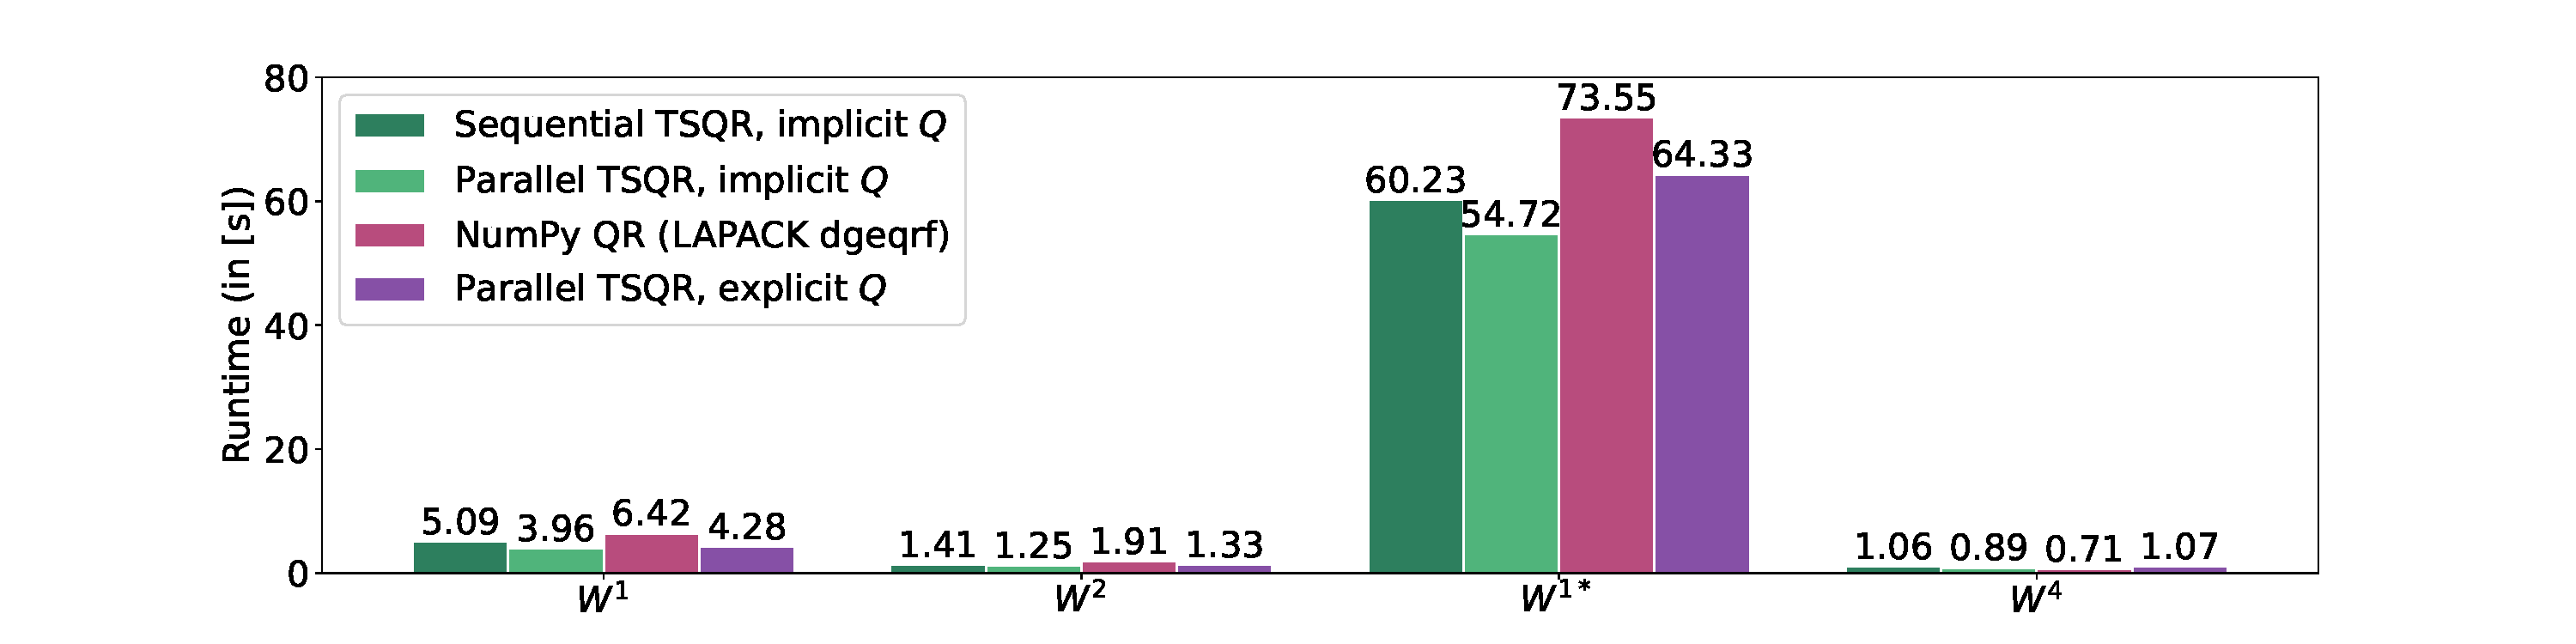
\includegraphics[width=\textwidth, trim = 0cm 1.5cm 0cm 1cm]{./plots/TSQR_Performance.pdf}
\end{figure}

\subsection{Numerical Stability of TSQR}

As already mentioned, we use the NumPy in-built function
\textit{numpy.linalg.qr} as a subroutine for our TSQR algorithms. This function
is an interface to the LAPACK routine \textit{dgeqrf} which uses Householder
$QR$. Similar to MGS, Householder $QR$ gives backward stable solutions
\cite{Bornemann:2018}. Moreover, Householder $QR$ is unconditionally stable
\cite{Grigori:2008}, i.e. the computed $Q$ factors are always orthogonal to
machine precision independent of the input matrix $W$: $||I - Q^T Q||_2 = O(u)$.
Our TSQR algorithms are composed of multiple $QR$ decompositions. Since these
factorizations are unconditionally stable, sequential and parallel TSQR are also
unconditionally stable. The orthogonality loss as well as the condition
$\kappa(Q)$ for our test matrices $W^1$, $W^2$, $W^{1^*}$ and $W^4$ can be found
in Table \ref{tab:errorOrthoTSQR}. In Figure \ref{fig:orthoErrorTSQR}, we plot
the orthogonality loss and $\kappa(Q)$ for the sequence of test matrices
generated by the procedure described in Section \ref{section:cgsStability}. As
expected, NumPy QR and both TSQR algorithms produce results that are orthogonal
to the machine precision independent of the given matrix. Furthermore,
$\kappa(Q)$ is $1$ for all matrices.
\begin{table}[t]
    \centering
    \caption{Orthogonality Error $||I - Q^T Q||_2$ of TSQR (loss scaled by $10^{-14}$)}
    \label{tab:errorOrthoTSQR}
    \renewcommand{\arraystretch}{1.2}
    \begin{tabular}{|p{2cm}|c|c|c|c|c|c|c|c|}
      \hline
      \multirow{2}{2cm}{\textbf{Algorithm}} & \multicolumn{2}{c|}{$\textbf{W}^1$} &
      \multicolumn{2}{c|}{$\textbf{W}^2$} & \multicolumn{2}{c|}{$\textbf{W}^{1^*}$} &
      \multicolumn{2}{c|}{$\textbf{W}^4$}\\
      \cline{2-9}
      & loss & $\kappa(Q)$ & loss & $\kappa(Q)$
      & loss & $\kappa(Q)$ & loss & $\kappa(Q)$\\
      \hline
      Sequential    & $1.39$ & $1$ & $1.39$ & $1$
                        & $3.05$ & $1$ & $1.41$ & $1$ \\ \hline
      Parallel      & $1.35$ & $1$ & $1.45$ & $1$
                        & $2.99$ & $1$ & $1.38$ & $1$ \\ \hline
      NumPy $QR$    & $1.27$ & $1$ & $1.33$ & $1$
                        & $3.16$ & $1$ & $1.01$ & $1$ \\ \hline
    \end{tabular}
  \end{table}

\begin{figure}[t]
    \centering %
    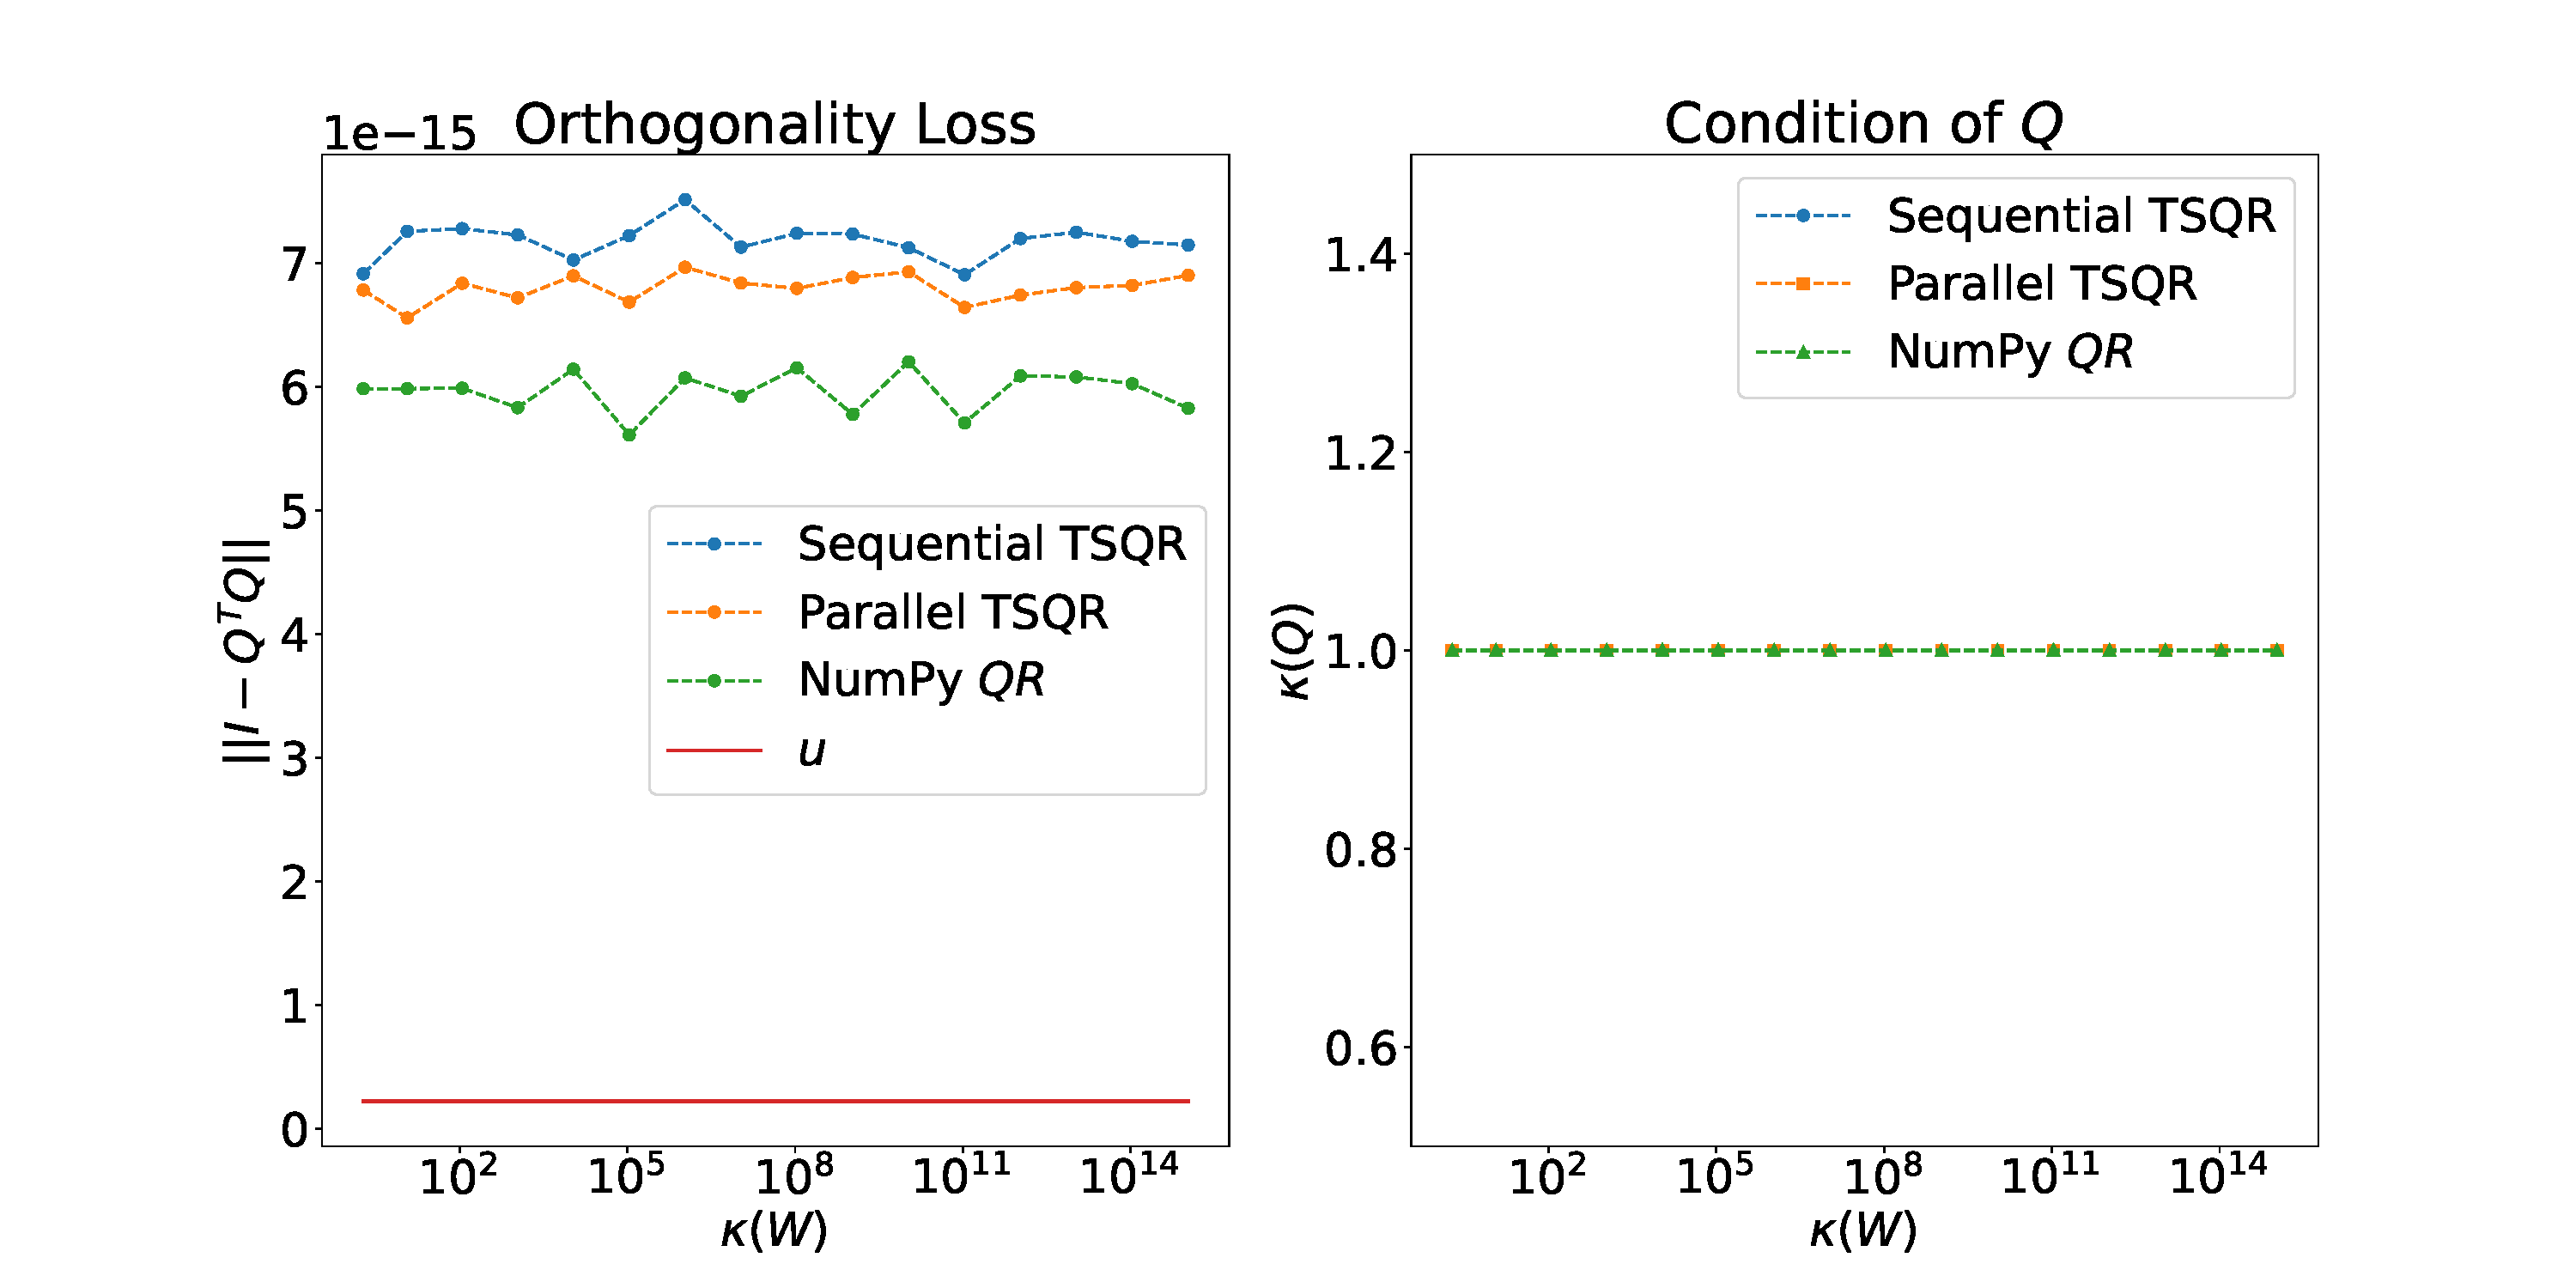
\includegraphics[width=\textwidth, trim = 0cm 0cm 0cm 1cm]
        {./plots/TSQR_Orthogonality_Error_complete.pdf}
    \caption{TSQR - Orthogonality loss and $\kappa(Q)$ as function of $\kappa(W)$}
    \label{fig:orthoErrorTSQR}
\end{figure}

\section{Conclusion}
To conclude, TSQR is the best choice for parallelizing the $QR$ decomposition of
tall and skinny matrices. In contrast to CGS and MGS, it is unconditionally
stable and the number of required messages scales independently of the matrix
size ($\#$ messages $\dot{=} \ \log(P)$). As the theory predicted, CGS was so
unstable in our experiments that it is not useful in practice. MGS is backward
stable but the orthogonality error still scales linearly with the condition of
the matrix. Although CGS and MGS require the same amount of floating point
operations, MGS is much slower in practice than CGS. An advantage of CGS and MGS
is that the already computed vectors in each iteration form an orthonormal
basis. In particular, each vector $q_i$ can be obtained after the $i$-th
iteration. In contrast, when using TSQR or Householder $QR$ one has to wait
until the completion of the algorithm to obtain any orthonormal vector. The
amount of messages sent while executing CGS or MGS scales linearly with the
number of columns of the input matrix and the corresponding lower bound for both
algorithms is $2n \log(P)$ \cite{Grigori:2008}.

\clearpage{}
\bibliographystyle{plainnat}
\bibliography{biblio}

\end{document}
